% Chapter3

\chapter{Grundlagen} \label{chapter:grundlagen}

%\begin{quotation}
%``The market is not an invention of capitalism. It has existed for centuries. It is an invention of civilization.``
%\begin{flushright}
%(Mikhail Gorbachev)
%\end{flushright}
%\end{quotation}

Aufgabe dieses Kapitels ist es zun�chst ein Fundament f�r das Verst�ndnis dieser Arbeit zu legen und Funktionsweisen, Vorg�nge sowie verschiedene Ans�tze zu erl�utern.\\

\section{Finanzwirtschaftliche Grundlagen}

% !TEX root = ../../Noctua_Diplomarbeit.tex

\subsection{Boerse und Preisbildung}

Eine B�rse ist ein Handelsmarkt, auf dem sich Preise durch Angebot und Nachfrage von Handelspartnern bilden und der Handel nicht direkt zwischen K�ufern und Verk�ufern, sondern �ber berechtigte H�ndler abgewickelt wird. Wichtig ist dabei, dass immer f�r ausreichend Liquidit�t gesorgt werden muss, so dass jederzeit Wertpapiere gekauft und auch verkauft werden k�nnen.

Handelsvorg�nge oder Trades resultieren aus einer Erwartungshaltung der Marktteilnehmer.  \cite{boerse-wien-funktion} \cite{boerse-frankfurt-funktion}
Unter der Annahme von steigenden Kursen werden Einheiten gekauft, i.e. es wird "`long gegangen"', werden fallende Kurse erwartet, werden entweder existierende St�ckzahlen verkauft oder es wird sogar ein Leerverkauf get�tigt, i.e. eine Short-Position er�ffnet. Damit wird der Verkauf von geborgten Wertpapieren bezeichnet, die zu einem sp�teren Zeitpunkt beim Schlie�en der Short-Position erst gekauft werden. Sinken die Kurse dazwischen, wird daher zu einem h�heren Preis verkauft als sp�ter gekauft wird und es entsteht die Differenz als Gewinn. \cite{gabler-leerverkauf}

Wollen mehr Handelsteilnehmer oder \emph{Trader} kaufen als verkaufen, steigt der Preis aufgrund der hohen Nachfrage, man spricht auch von einem Bullenmarkt. \cite{duden-bullenmarkt}
Ist es andersherum so, dass die Verk�ufer �berwiegen und der Preis sinkt, handelt es sich um einen B�renmarkt. \cite{duden-baerenmarkt}\\

F�r jedes Wertpapier wird ein sogenanntes Orderbuch gef�hrt, das die aktuellen Kauf- und Verkaufsauftr�ge beinhaltet. Investoren interessieren sich meist f�r die sogenannte Quote-Zeile, die Informationen zu den g�nstigsten Konditionen sowohl auf K�ufer- als auch auf Verk�uferseite bietet.\\

Eine Quote-Zeile von Apple (AAPL) k�nnte dabei folgenderma�en aussehen.

\begin{center}
\begin{tabular}{|c|c|c|c|}
\hline 
Bid & Bid Size & Ask & Ask Size \\ \hline
691.52 & 7 & 691.66 & 3 \\ \hline
\end{tabular}
\end{center}

Der Bid-Preis von \textdollar{691.52} ist das h�chste vorhandene Gebot f�r eine Apple-Aktie. Die Bid-Size gibt die Information �ber die Anzahl an Aktien, die K�ufer zu diesem Preis erstehen wollen. Die Anzahl wird in \emph{round lots} angegeben; meist entspricht ein Round Lot 100 St�ck der Aktie. Die Bid-Seite beschreit somit die K�uferseite. Der Ask-Preis und die Ask-Size beschreibt hingegen das beste Angebot auf der Verk�uferseite. In diesem Fall werden 3 Round Lots f�r den St�ckpreis von \textdollar{691,66} pro Aktie angeboten. Ein Round Lot w�rde in diesem Fall also \textdollar{69166,00} kosten.

Soll ein Handel schnellstm�glich abgewickelt werden muss zum Ask-Preis gekauft und zum Bid-Preis verkauft werden. Wird in diesem Fall mindestens die Ask- bzw. Bid-Size gehandelt, ver�ndert sich die Quote-Zeile so, dass das n�chstbeste Angebot angezeigt wird. Diese Hintereinanderreihung von Angeboten wird auch als Orderbuchtiefe bezeichnet. \\
Angenommen, ein K�ufer ist nicht bereit zum aktuellen Ask-Preis zu kaufen. Er will bessere Konditionen und schickt eine \emph{Limit-Order}, d.h. zu gegebenem Preis oder besser \footnote{IB-Ordertypen siehe: http://www.interactivebrokers.com/de/p.php?f=orderTypes}, mit einem Limit, das zwischen Ask- und Bid-Preis liegt. Sein Kaufgebot ist damit h�her als der zuvor h�chste und wird daher sofort in der Quote-Zeile auf der Bid-Seite angezeigt.

Der Aktienkurs wird mithilfe dieser vorhandenen Orders so gebildet, dass stets der h�chste Umsatz entsteht. Bei hoher Nachfrage auf K�uferseite steigt dadurch der Preis, dominieren jedoch die Verk�ufer sinkt dieser. \cite{charttec-kursfeststellung}
% !TEX root = ../../Noctua_Diplomarbeit.tex

\subsection{Markt und Marktzust�nde}

Aktienpreise setzen sich vollst�ndig aus Angebot und Nachfrage zusammen. Nachfrage entsteht, wenn Handelsteilnehmer annehmen, dass die Preise steigen, Angebot durch die Erwartung von negativen Kursverl�ufen.
Diese Annahmen beruhen auf einer Vielzahl von Informationen, die zur Verf�gung stehen. Somit haben diese Informationen einen direkten Einfluss auf die Aktienkurse. Ver�ffentlicht ein Unternehmen seine Bilanz und fallen darin die Gewinne h�her aus als erwartet, wird der Aktienkurs aufgrund dieser Information steigen. Die Preise reflektieren aber nicht nur realisierte Gewinne, sondern auch potentiell zuk�nftige. W�ren in der Theorie alle m�glichen Informationen allen Handelsteilnehmern bekannt, w�rde sich der Kurs nur mehr durch das Auftauchen von neuen Informationen ver�ndern. In der Praxis verh�lt es sich anders, da weder alle Informationen vorhanden sind, noch Handelsteilnehmer absolut rational agieren.

Diese in den 1960er-Jahren entwickelte Theorie wird als \emph{Efficient Market Hypothesis} bezeichnet und besagt kurz gefasst, dass Marktpreise alle verf�gbaren Informationen vollst�ndig widerspiegeln.\\
Au�er der Schlussfolgerung, dass Nachrichten und Ereignisse f�r Preisentwicklungen h�chst relevant sind, l�sst sich ebenfalls folgern, dass positive Informationen, z.B. eine Wachstumsprognose, keinen Kursanstieg bedeuten m�ssen, weil diese Informationen schon im aktuellen Marktpreis enthalten sein k�nnen. \cite{lo-efficient-market-hypothesis}\\
Unter der Pr�misse, dass die Efficient Market Hypothesis uneingeschr�nkte G�ltigkeit besitzt, l�sst sich au�erdem deduzieren, dass zuk�nftige Preise nicht vorhersehbar sind. W�re dies n�mlich der Fall und k�nnte jeder Markteilnehmer die Preise beliebig genau vorhersagen, w�re niemand bereit, unter dem vorhergesagten Preis zu verkaufen und niemand w�rde dar�ber kaufen. Daraus resultiert, dass der Aktienmarkt den vorhergesagten Preis fixiert. Da nur neue Informationen, die noch nicht bekannt sind, das Preisniveau ver�ndern, sind folglich auch die Preise noch nicht bekannt. \cite{bodie-investments}\\

Da ein Marktpreis bei erh�hter Nachfrage steigt, ist es f�r Aktienanleger sinnvoll, Geld dort anzulegen, wo auch andere investieren. Ein Vorteil liegt daher darin, herauszufinden, was die Mehrheit oder der Markt denkt und nicht in der pers�nlichen Einsch�tzung des Wertes. John Maynard Keynes beschreibt diese Theorie schon 1936 in seiner \emph{General Theory}.\\
In dieser Theorie l�sst sich eine R�ckkopplung zur Information erahnen. Nicht nur die urspr�ngliche Information selbst spielt eine Rolle, sondern auch die Reaktion darauf, im Falle von Aktien also die Kursentwicklung. Dieser iterative Prozess ben�tigt aufgrund von menschlichem Handeln aber auch seine Zeit. Deshalb entstehen durch Kursschwankungen und die verursachten Reaktionen Trendbewegungen in den M�rkten. Erst durch diesen eigentlich psychologischen Effekt funktionieren Charttechniken und technische Analysen.\\
F�r jene, die sich zus�tzlich noch mit makro�konomischen Zusammenh�ngen befassen, besteht trotzdem weiterhin ein Vorteil. Marktr�ckkopplungen unterliegen einem "`Herdentrieb"' und k�nnen zu Spekulationsblasen f�hren. �bergeordnete Vorg�nge k�nnen somit fr�hzeitige Hinweise liefern und bei der korrekten Interpretation der resultierenden Kursverl�ufe helfen. \cite{singer-herdentrieb}

Um die Performance von Trendfolgemethoden zu optimieren, sollen verschiedene Marktzust�nde unterschieden werden, die sich auf den Kursverlauf auswirken. Zu diesem Zweck k�nnen diverse Kriterien untersucht werden, angefangen bei unterschiedlich langen Trendverl�ufen, pl�tzliche Kursbewegungen, Dauer eines Trends usw.\\
Beispielsweise k�nnte sich herausstellen, dass bei einem sehr langfristigen Aufw�rtstrend bei Kaufsignalen die Long-Positionen immer gr��er ausfallen sollten als die Short-Positionen bei Verkaufssignalen oder dass erh�hte Volatilit�t einen Kurseinbruch oder eine Trendumkehr ank�ndigen.\\

\begin{figure}
	\centering
		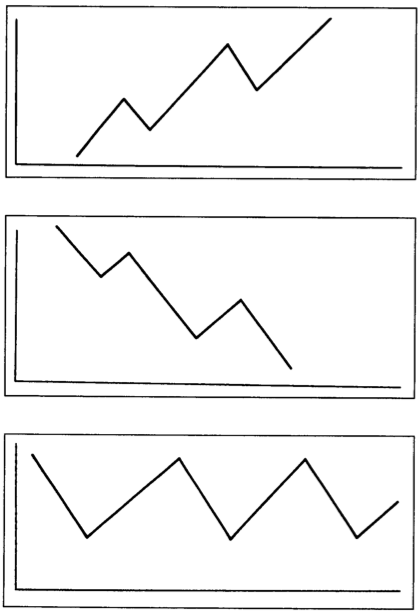
\includegraphics[width=0.8\textwidth]{graphics/fingrundlagen/trend_types.png}
	\caption[Typen von Trends]{Typen von Trends: Aufw�rts-, abw�rts und seitw�rts gerichteter Markt \cite{murphy-technische}}
	\label{fig:trend_types}
\end{figure}

Bei der Trendbestimmung in B�rsenkursen gelten gleitende Durchschnitte, oder \glspl{ma}, als ein beliebtes Mittel und infolge dessen h�ufig genutzter Indikator. Die klassische technische Analyse ist oft subjektiv und unterliegt einem gewissen Interpretationsspielraum, w�hrend algorithmische Handelssysteme klare Entscheidungen generieren m�ssen, weshalb einerseits immer wieder Fehlentscheidungen getroffen werden, andererseits das Handelssystem ausreichend viele Faktoren einbeziehen sollte.

Ein \gls{ma} ist, wie der Name bereits verr�t, eine Art statistischer Durchschnitt einer Reihe von Werten. "`Gleitend"' oder "`moving"' bedeutet, dass nicht alle historischen Daten in die Durchschnittsberechnung einflie�en, sondern nur eine beschr�nkte Anzahl der vergangenen Daten. Es gibt unterschiedliche Varianten von \glspl{ma}, die sich darin unterscheiden wie viele historische Daten verwendet werden und wie die einzelnen Datens�tze gewichtet werden. Klassisch werden Schlusskurse zur \gls{ma}-Berechnung verwendet, wobei manche Trader es vorziehen, Open- oder Mittelwerte aus Open- und Close heranzuziehen. Eine weitere Variante ist eine sepa\-rate Berechnung von \glspl{ma} f�r High- und Low-Kurse, wodurch ein Band entsteht, das eine Art Neutralbereich anzeigt, der beispielsweise als Signalfilter verwendet werden kann. Prinzipiell sind alle \glspl{ma} Trendfolge-Indikatoren, sie antizipieren keine zuk�nftigen Kursver�nderungen, wie viele andere Methoden der technischen Analyse, sondern reagieren nur auf bereits stattgefundene Trendwenden.\\
% !TEX root = ../../Noctua_Diplomarbeit.tex

\subsection{Unterst�tzung und Widerstand}

Die Kurse von Aktien unterliegen, wie bereits erw�hnt, gewissen Trends, die entweder auf-, ab- oder auch seitw�rts (weder auf- noch abw�rts) verlaufen. Bei steigenden Kursen erreichen diese irgendwann ein Level, bei dem der Preis nicht mehr als billig angesehen wird und der Kurs dreht sich um. Der Trend verliert also seine Nachhaltigkeit. Dieses Level wird als \emph{Widerstand} oder \emph{Resistance} bezeichnet, da es nur schwer �berwunden wird. Sinkt der Kurs eine Weile wieder und sonstige Bewertungskriterien des Handelsgutes haben sich nicht signifikant ver�ndert, erreicht der Kurs einen Punkt, bei dem er wieder interessant f�r etwaige K�ufer wird. Diese Schwelle wird als \emph{Unterst�tzung} oder \emph{Support} bezeichnet. \cite{elder_living} Am Beispiel von Microsoft kann diese Funktion in der Abbildung \ref{fig:msft_sup_res} �ber einen l�ngeren Zeitraum beobachtet werden\\

Diese beiden Schwellen sind tempor�re Hilfsmittel und lassen Wendepunkte erahnen. Beim Durchbruch eines Levels kann hingegen mit einer Fortsetzung dieses Trends gerechnet werden und ggf. wird ein alter Widerstand zur Unterst�tzung. \cite{investopedia-support-resistance} Abbildung \ref{fig:payx_sup_res} von Paychex Inc. veranschaulicht diesen Wechsel von Unterst�tzungs- zu Widerstands- und wieder zur�ck zu Unterst�tzungsleveln.

\begin{figure}
	\centering
		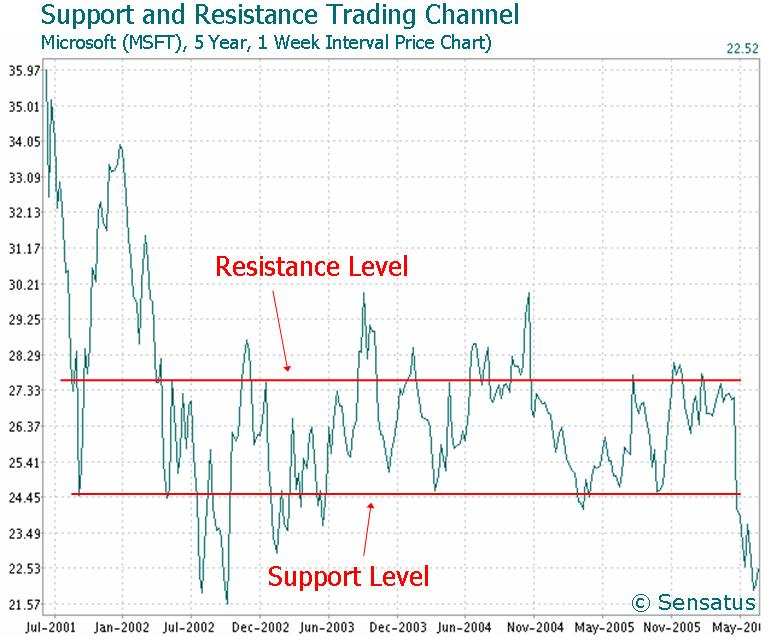
\includegraphics[width=0.8\textwidth]{graphics/fingrundlagen/msft_sup_res.JPG}
	\caption[Microsoft Support Resistance]{Microsoft 5-Jahres-Chart mit 1-Wochen-Intervallen und eingezeichneten Support- und Resistance-Leveln}
	\label{fig:msft_sup_res}
\end{figure}

\begin{figure}
	\centering
		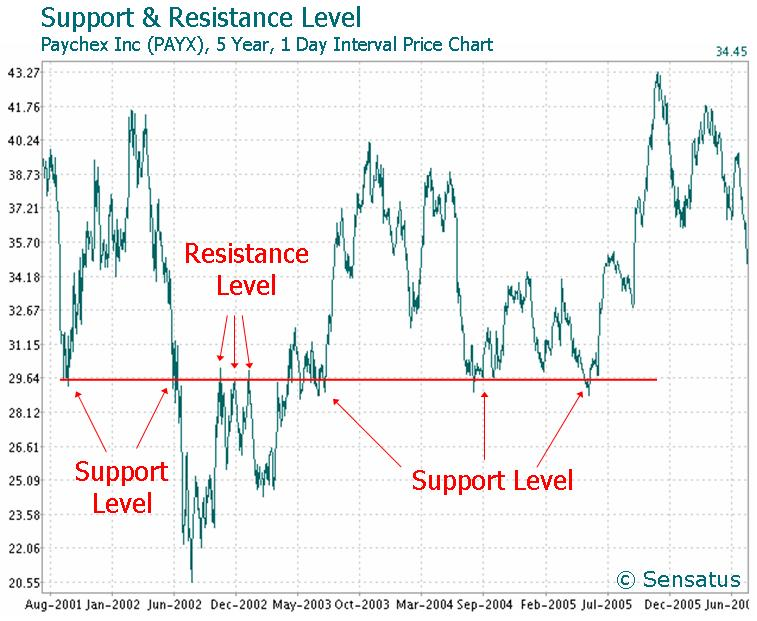
\includegraphics[width=0.8\textwidth]{graphics/fingrundlagen/payx_sup_res.JPG}
	\caption[Paychex Inc. Support Resistance]{Paychex Inc. 5-Jahres-Chart mit 1-Wochen-Intervallen; Level wechselt zwischen Support- und Resistance-Funktion}
	\label{fig:payx_sup_res}
\end{figure}
% !TEX root = ../../Noctua_Diplomarbeit.tex

\subsection{Indikatoren} \label{Indikatoren}

%%%%%%%%%%%%%%%%%%%%%%%%%%%%%%%%%%%%%%%
\subsubsection{Simple Moving Average}

Die einfachste M�glichkeit, um Trends in Aktienkursen sichtbar zu machen, ist eine Gl�ttung des Preisverlaufs, also eine Art Durchschnittsberechnung.
Dadurch erh�lt man einen stabileren �berblick �ber die Richtung, in die sich der Kurs bewegt, ohne dass einmaligen Ausbr�chen zu viel Gewicht geschenkt wird.

Bei einem \gls{sma} wird f�r jeden neuen Wert jeweils aus den letzten $n$ Werten ein arithmetischer Mittelwert berechnet. Soll aus einer Reihe von Close-Kursen ein 10-Tages-\gls{sma} berechnet werden, werden dazu die letzten 10 Schlusskurse addiert und anschlie�end durch 10 dividiert, um einen Wert zu erhalten. F�r den folgenden Mittelwert wird der �lteste subtrahiert, ein weiterer neuer Wert addiert und die Summe anschlie�end wieder f�r einen Mittelwert durch 10 dividiert. Auf diese Weise entsteht ein gegl�tteter Kurs, der kurzzeitige Preisver�nderungen abschw�cht, wodurch Trends klarer erkennbar werden.

Zwei h�ufig kritisierte Eigenschaften des \gls{sma} sind, dass erstens nicht alle vorhandenen Daten in die Berechnung einbezogen werden und zweitens alle verwendeten Kursdaten mit gleicher Gewichtung in das Resultat eingehen. Bei einem 10-Tage-\gls{sma} hat jeder Kurswert, unabh�ngig vom Alter, eine Gewichtung von 10\%, bei einem 20-Tage-\gls{sma} 5\%.\\

Ein \gls{sma} wird wie folgt berechnet:

\begin{equation}
	\label{Simple Moving Average}
	P^{*}_t = \frac{1}{n} * \sum\limits_{i=0}^n{P_{t-i}}
\end{equation}

Dabei ist $P^{*}_t$ der gegl�ttete Wert zum Zeitpunkt $t$, $n$ die Anzahl an einbezogenen Werten und $P_{t-i}$ der Preis zum Zeitpunkt $t-i$. \cite{elder_living} \cite{murphy-technische}

\begin{figure}
	\centering
		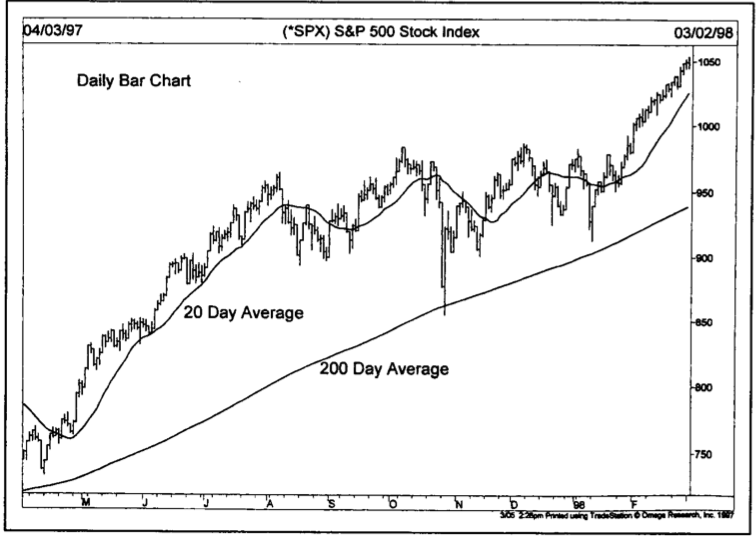
\includegraphics[width=0.8\textwidth]{graphics/fingrundlagen/sma.png}
	\caption[20- und 2-Tage SMA]{Vergleich eines 20- und 2-Tage SMA \cite{murphy-technische}}
	\label{fig:sma}
\end{figure}

%%%%%%%%%%%%%%%%%%%%%%%%%%%%%%%%%%%%%%%
\subsubsection{Linear Weighted Moving Average}

Um eines der Probleme des \gls{sma} zu vermeiden, n�mlich die gleiche Gewichtung aller Daten �ber die Zeit, kann ein \gls{lwma} verwendet werden. Dabei werden Daten zu fr�heren Zeitpunkten geringer gewichtet, als aktuellere Daten. Konkret wird der neueste Eintrag mit $n$ multipliziert, der vorangehende mit $n-1$ und so weiter bis der letzte den Multiplikationsfaktor 1 erh�lt. Die daraus gebildete Summe muss anschlie�end noch durch die Summe der Multiplikatoren dividiert werden, um einen Durchschnitt zu erhalten. Bei einem 10-Tage-\gls{lwma} werden die Kursdaten von neu nach alt mit $10, 9, 8, 7,\dots, 1$ multipliziert und die anschlie�end gebildete Summe durch $10+9+8+7+\dots+1$ dividiert.

\begin{equation}
	\label{Linear Weighted Moving Average}
	P^{*}_t = \frac{\sum\limits_{i=0}^{n-1}{P_{t-i} * (n-i)}}{\sum\limits_{i=0}^{n-1}{i}}
\end{equation}

$P^{*}_t$ ist hier wiederum der gegl�ttete Preis zum Zeitpunkt $t$, $P_t$ der Preis zum Zeitpunkt $t$. \cite{murphy-technische}

%%%%%%%%%%%%%%%%%%%%%%%%%%%%%%%%%%%%%%%
\subsubsection{Exponential Moving Average}

Der \gls{ema} versucht beide Hauptkritikpunkte am \gls{sma} zu l�sen, indem er neuere Werte immer st�rker gewichtet und alle zur Verf�gung stehenden Daten in die Berechnung einbezieht. Man spricht auch vom exponentiell gegl�tteten gleitenden Durchschnitt. Dazu muss ein \emph{\gls{sf}}, auch Gl�ttungsfaktor genannt und meist als $\alpha$ bezeichnet, zwischen 0 und 1 gew�hlt werden, mit dem ein neuer Wert multipliziert wird. Der vorherige Wert wird mit der Differenz des \gls{sf} zu 1 multipliziert. Der aktuelle Wert des \gls{ema} ergibt sich dann aus der Addition dieser beiden gewichteten Werte. Dadurch bleibt jeder Kurswert unendlich lange in der weiteren Berechnung bestehen, die Bedeutung �lterer Kurswerte konvergiert jedoch gegen 0. Aus ebendiesem Grund handelt es sich, mathematisch rigoros betrachtet, beim \gls{ema} nicht wirklich um einen \emph{moving} average, da sich der Wertebereich nicht verschiebt, sondern immer alle Werte zur Berechnung verwendet werden. \cite{klinker-exponential}

Um exponentielle Durchschnittswerte mit normalen \gls{ma}-Werten vergleichen zu k�nnen, wird $\alpha$ meist mit einer Formel berechnet, die n�herungsweise die gleiche Periode f�r ein bestimmtes $n$ ergibt.

\begin{equation}
	\label{Gl�ttungsfaktor alpha}
	\alpha = 2/(n+1)
\end{equation}
	
Soll nur der aktuelle Wert berechnet werden, ist eine rekursive Berechnung naheliegend. Eine m�glichst performante Berechnung einer exponentiell gegl�tteten Zeitreihe beginnt meistens mit einem arithmetischen Mittel �ber die ersten $n$ Werte, um einen Anfangswert zu erhalten, der einen \gls{ema}-Wert besser approximiert, als wenn der erste Preis als Anfangswert herangezogen w�rde.

Die folgende Formel soll die Berechnung des exponentiell gegl�tteten Preises $P^{*}_t$ zum Zeitpunkt $t$ verdeutlichen. Dabei ist $\alpha$ der \gls{sf} und $P^{*}_{t-1}$ der exponentiell gegl�ttete Preis zum Zeitpunkt $t-1$.

\begin{equation}
	\label{Exponential Moving Average}
	P^{*}_t = \alpha * P_{t} + (1 - \alpha) * P^{*}_{t-1}
\end{equation}
\cite{murphy-technische} \cite{elder_living}

\begin{figure}
	\centering
		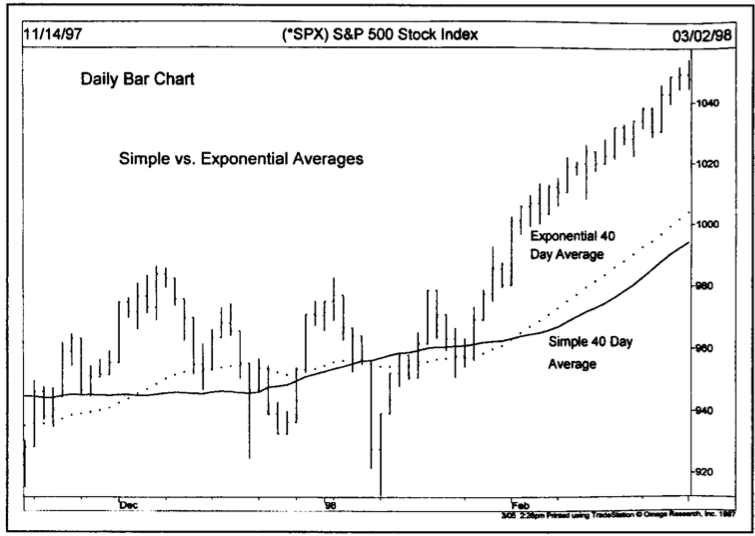
\includegraphics[width=0.8\textwidth]{graphics/fingrundlagen/sma_ema}
	\caption[Vergleich SMA mit EMA]{Vergleich eines 40-Tage SMA mit einem 40-Tage EMA \cite{murphy-technische}}
	\label{fig:sma_ema}
\end{figure}

%%%%%%%%%%%%%%%%%%%%%%%%%%%%%%%%%%%%%%%
\subsubsection{Double und Triple Exponential Moving Average}

Um den Lag, also das Hinterherhinken der gegl�tteten Zeitreihe hinter dem tats�chlichen Kurs, zu reduzieren, gibt es die M�glichkeit, neue Daten noch st�rker zu gewichten als bei einem normalen \gls{ema}.
1994 von Patrick Mulloy eingef�hrt, schaffen sowohl der \gls{dema} als auch der noch st�rker neue Daten gewichtende \gls{tema} bei dieser Problematik Abhilfe.
Den \gls{dema} darf man sich allerdings nicht als \gls{ema} eines bereits berechneten \gls{ema} vorstellen. Das w�rde zu einer unerw�nschten starken Abwertung aktueller Daten f�hren, wie an den Gewichtungsgraphen in Abbildung \ref{fig:wrong_dema_tema} zu sehen ist. Tats�chlich wird der \gls{dema} aus einer Zusammensetzung aus einem einfachen und einem doppelten \gls{ema} berechnet, wodurch ein neuer \gls{ma} mit weniger Lag als jede der Komponenten entsteht. \cite{mulloy-smoothing}

\begin{equation}
	\label{Double Exponential Moving Average}
	DEMA = 2*EMA - EMA(EMA)
\end{equation}

\begin{equation}
	\label{Triple Exponential Moving Average}
	TEMA = 3*EMA - 3*EMA(EMA) + EMA(EMA(EMA))
\end{equation}

\begin{figure}[htbp]
	\centering
	\begin{minipage}[b]{0.4\textwidth}
		\centering
 			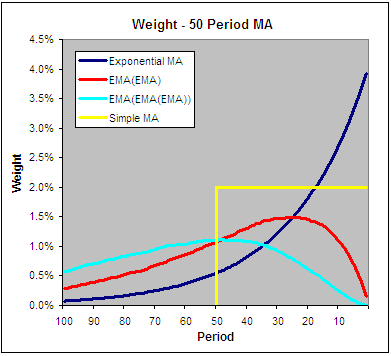
\includegraphics[width=0.9\textwidth]{graphics/chapter2/fingrundlagen/wrong_dema_tema.png}
			\caption[Falsche Multiple Exponential Average Gewichtung]{Falsche Double und Triple Exponential Average Gewichtung}
			\label{fig:wrong_dema_tema}
	\end{minipage}\hspace{0.01\textwidth}	% Abstand zwischen den Bildern = 1% der Textbreite
	\begin{minipage}[b]{0.4\textwidth}
		\centering
 			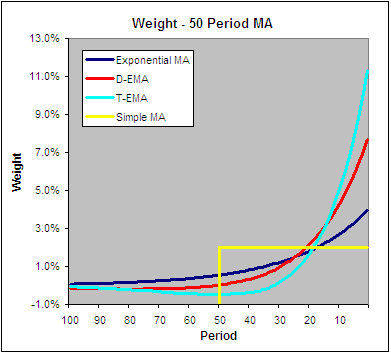
\includegraphics[width=0.9\textwidth]{graphics/chapter2/fingrundlagen/right_dema_tema.png}
			\caption[Richtige Multiple Exponential Average Gewichtung]{Richtige Double und Triple Exponential Average Gewichtung}
			\label{fig:right_dema_tema}
	\end{minipage}
\end{figure}

\cite{etf-hq-dema-tema}

%%%%%%%%%%%%%%%%%%%%%%%%%%%%%%%%%%%%%%%
\subsubsection{MACD}

Der \gls{macd} ist ein Indikator zur Darstellung der Differenz zwischen zwei \glspl{ema}. Der l�ngere \gls{ema} wird vom k�rzeren abgezogen, um bei einem Kreuzungspunkt genau einen Wert von 0 zu erhalten. Eine andere M�glichkeit eines \gls{macd}-basierten Handelssystems ist, den \gls{macd} mit einem zus�tzlichen \gls{ema} zu vergleichen, der k�rzer ist als beide zur Berechnung des \gls{macd} verwendeten \glspl{ema}. Dies wird als Signallinie bezeichnet. Obwohl die Signallinie den k�rzesten Zeitraum abbildet, ist der \gls{macd} n�her am tats�chlichen Kurs. Wenn der \gls{macd} die Signallinie von unten schneidet, entspricht dies daher einem Kaufsignal und umgekehrt. \cite{elder_living}

\begin{figure}
	\centering
		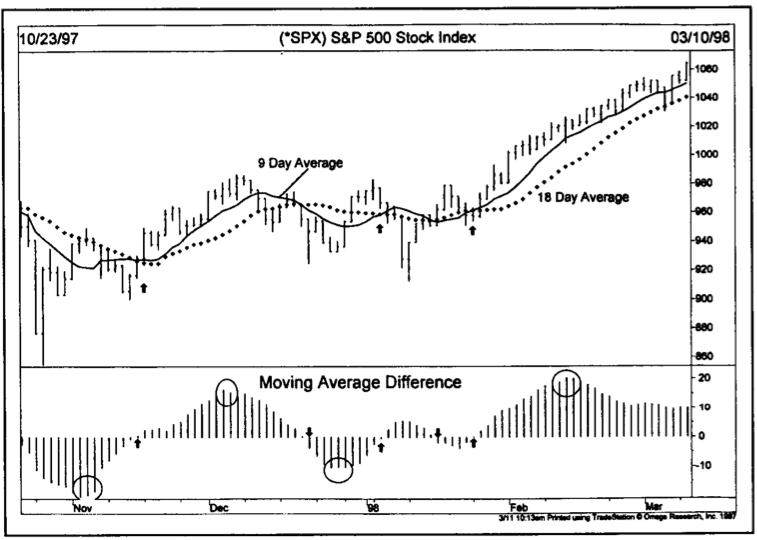
\includegraphics[width=0.8\textwidth]{graphics/fingrundlagen/macd.png}
	\caption[9,18 MACD-Histogramm]{9,18 MACD-Histogramm am Beispiel des S\&P 500 \cite{murphy-technische}}
	\label{fig:macd}
\end{figure}

%%%%%%%%%%%%%%%%%%%%%%%%%%%%%%%%%%%%%%%
\subsubsection{AMA}

Ein Problem des \gls{ema} ist es, die bestm�gliche L�nge zu w�hlen, um einen m�glichst aussagekr�ftigen Durchschnitt zu erhalten. Perry Kaufman schl�gt eine variable L�nge als L�sung des Problems vor. Dabei wird der Gl�ttungsfaktor eines \gls{ema} anhand der Volatilit�t des Preises der letzten $n$ Perioden bestimmt. Der resultierende Indikator wird folglich \gls{ama} genannt. \cite{murphy-technische}

Kaufman bestimmt die Volatilit�t durch eine \gls{er}, die berechnet wird, indem die absolute Gesamtpreisbewegung, i.e. Preis am Ende der Periode abz�glich des Preises am Beginn, durch die Summe der absoluten Preisbewegungen in einer Periode dividiert wird. Aufgrund der \gls{er} und zwei gegebenen L�ngen ($\alpha$ zwischen 0 und 1) wird nun ein tats�chlicher \gls{sf} berechnet. Dieser sollte zwischen den beiden gegebenen Werten liegen, was jedoch nur dann immer der Fall ist, wenn in der Berechnung des \gls{sf} $1$, nicht $2$ als Exponent gew�hlt wird.

\begin{equation}
	\label{Efficiency Ratio}
	ER = (\textrm{Gesamtpreisbewegung}) / (\textrm{Summe der Bewegungen pro Bar})
\end{equation}

\begin{equation}
	\label{Adaptive Moving Average - Smoothing Factor}
	SF = (ER * (SF_S - SF_L) + SF_L)^2
\end{equation}

\begin{equation}
	\label{Adaptive Moving Average}
	AMA_t = SF * P_{t} + (1 - SF) * AMA_{t-1}
\end{equation}

Dabei ist $SF_S$ der schnelle Smoothing Factor und $SF_L$ der langsame, zwischen denen das Ergebnis $SF$ abh�ngig von der $ER$ liegen soll.
Der Exponent kann als Abwandlung des Indikators auch ver�ndert werden, beispielsweise auf $1$, wenn der resultierende Durchschnitt genau im angegebenen Bereich liegen soll, oder auch auf $0.75$, falls konservativere Durchschnitte erw�nscht sind. \cite{kaufman_systems} \cite{ama_whs}

%%%%%%%%%%%%%%%%%%%%%%%%%%%%%%%%%%%%%%%
\subsubsection{Lineare Regression}

Um aus Zeitreihen einen allgemeinen Trend erkennen zu k�nnen, wird h�ufig eine lineare Regression durchgef�hrt. Dabei wird eine Gerade so gelegt, dass alle Punkte so nahe wie m�glich an
der Geraden liegen, wobei alle Punkte gleich stark gewichtet werden und auch m�glichst gleich weit entfernt liegen sollen. Zur Abstandsmessung werden die quadrierten y-Abst�nde zwischen Gerade und Preis herangezogen, damit gr��ere Abst�nde st�rker gewichtet werden als kleine. Die Gerade wird nun so gelegt, dass diese Summe der quadratischen Abst�nde m�glichst klein ist.

Das Minimum der folgenden Funktion der quadratischen Abst�nde muss durch partielles Differenzieren gefunden werden.

\begin{equation}
	\label{Funktion der quadratischen Abst�nde}
	F(k,d) = \sum\limits{i=1}{n}{{k*x_i + d - y_i}^2}
\end{equation}

Dadurch erh�lt man $k$ und $d$ der Regressionsgeraden. In der praktischen Anwendung ist meist besonders die Steigung $k$ der Geraden relevant.
Wird die Anzahl an historischen Preisen variiert, erh�lt man so Richtung und St�rke verschieden langer Trends.

%%%%%%%%%%%%%%%%%%%%%%%%%%%%%%%%%%%%%%%
\subsubsection{Average Directional Index}\label{subsection:adx}

Der \gls{adx} ist ein Indikator, der es auf einfache Weise erm�glicht, die St�rke eines Trends zu bestimmen, jedoch nicht, ob es sich um einen Aufw�rts- oder Abw�rtstrend handelt. Er wurde Ende der Siebziger von Welles Wilder entwickelt, der u.a. auch f�r den RSI (s. \ref{subsubsection:rsi}) verantwortlich ist. Der \gls{adx} ist ein Indikator, der sich aus der True Range (TR) und den Directional Movement-Indikatoren $DM_+$ und $DM_-$ zusammensetzt. Alle zusammen werden auch als Directional System bezeichnet. \cite{atr_whs} \cite{elder_living}

Der \gls{adx} wird in 5 Schritten berechnet.

\begin{enumerate}
	\item{Directional Movement ($DM_+$, $DM_-$) berechnen\\
		Directional Movement bezeichnet die Spanne, in der sich der Preis in der aktuellen Periode �ber oder unter der Preisspanne der letzten Periode bewegt hat.
		$DM_+$ ist dabei die Spanne dar�ber, $DM_-$ jene darunter. Der $DM$ ist dabei immer positiv, es wird also der Betrag der Differenz verwendet. (siehe Abbildung \ref{fig:dm})}
	\item{True Range ($TR$) berechnen\\
		Die True Range soll die tats�chliche Preisbewegung abbilden, also auch Bewegungen zwischen Perioden, bei denen Close- und Open-Preise
		nicht ident sind. Daf�r wird f�r die $TR$ immer der gr��te der folgenden 3 Werte herangezogen, die sich aufgrund von Preisen des aktuellen und 
		vorhergehenden Bars berechnet.
		\begin{enumerate}
			\item{$\left|\textrm{Aktuelles Hoch} - \textrm{Aktuelles Tief}\right|$}
			\item{$\left|\textrm{Aktuelles Hoch} - \textrm{Vorheriges Tief}\right|$}
			\item{$\left|\textrm{Aktuelles Tief} - \textrm{Vorheriges Tief}\right|$}
		\end{enumerate}}
	\item{Directional Indicators ($DI_+$, $DI_-$) berechnen\\
		 Die Directional Indicators sind das Verh�ltnis der Trendbewegung zur True Range, es gilt also:\\
		\begin{equation}
			DI_+ = \frac{DM_+}{TR}
		\end{equation}
		\begin{equation}
			DI_- = \frac{DM_-}{TR}
		\end{equation}}
	\item{Directional Indicators gl�tten\\
		Die Directional Indicators ($DI_{n+}$ und $DI_{n-}$) erh�lt man, indem die Directional Indicators ($DI_+$, $DI_-$) mit einem \gls{ma} gegl�ttet werden,
		wof�r in der Regel ein \gls{ema} verwendet wird. Die L�nge des verwendeten \gls{ma} ist dabei auf die Tradingstrategie anzupassen.
		$DI_{n+}$ und $DI_{n-}$ sind bereits f�r ein Handelssystem geeignet, da sie das Verh�ltnis von relativer Trendbewegung zur True Range gegl�ttet angeben.
		Aufgrund der Kreuzung der beiden Indikatoren k�nnen so auch Kauf- und Verkauf-Signale gegeben werden.}
	\item{$ADX$ berechnen\\
		Der \gls{adx} ist nun die nochmals gegl�ttete Differenz zwischen $DI_{n+}$ und $DI_{n-}$ und wird wie folgt berechnet:\\
		\begin{equation}
			ADX = EMA(\frac{DI_{n+} - DI_{n-}}{DI_{n+} + DI_{n-}})
		\end{equation}}
\end{enumerate} 

% V: Directional Movement Graph
\begin{figure}
	\centering
		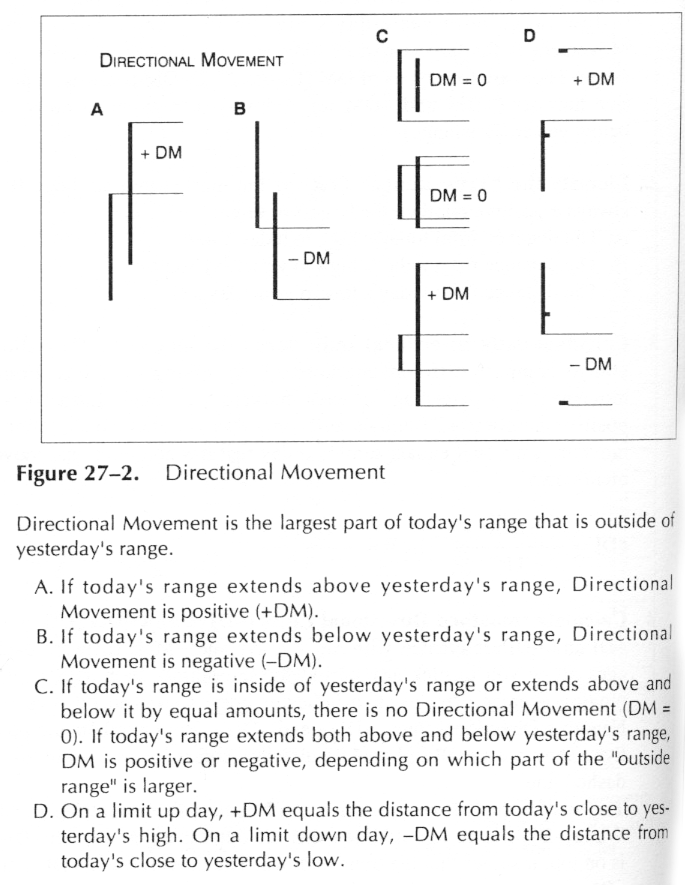
\includegraphics[width=0.8\textwidth]{graphics/fingrundlagen/dm.png}
	\caption[Berechnung des Directional Movement]{Berechnung des Directional Movement \cite{elder_living}}
	\label{fig:dm}
\end{figure}

Der \gls{adx} ist hilfreich, indem er anzeigt, ob sich der Markt in einer Trendphase befindet, in der Handelssysteme, die auf Trendfolgesystemen basieren, gut funktionieren, oder in einer Seitw�rtsphase,
in der sich andere Systeme eher rentieren. (z.B. Fading, siehe \ref{subsection:fading})  \cite{elder_living}

%%%%%%%%%%%%%%%%%%%%%%%%%%%%%%%%%%%%%%%
\subsubsection{Momentum}

Das Momentum ist ein Oszillator, der die Kurssteigung �ber einen gewissen Zeitraum angibt. Aus der Differenz des Preises zum Zeitpunkt $t$ und des Preises vor $n$ Perioden ergibt sich eine einfach interpretierbare Anzeige f�r die St�rke eines Trends. Aus einem 10-Tage-Momentum ist ablesbar, ob der Kurs aktuell h�her notiert als noch vor 10 Tagen. Wenn das Momentum negativ ist und ansteigt, ist ersichtlich, dass die St�rke eines aktuellen Abw�rtstrends abnimmt, wobei der Trend immer noch abw�rts gerichtet sein kann, er wird nur nicht mehr st�rker. Erst bei einem positiven Wert des Momentum ist ein Aufw�rtstrend zu erkennen.
Der gro�e Vorteil dieses Indikators liegt in der Fr�hzeitigkeit seiner Anzeige. Bevor sich der Trend umkehrt, zeigt der Momentum-Oszillator aufgrund der abnehmenden St�rke des aktuellen Trends bereits an, dass ein Trendwechsel bevorstehen k�nnte. Ein Problem des Momentum ist, dass die Werte absolut berechnet werden und dadurch die Schwankungsbreite abh�ngig vom betrachteten Kurs stark variieren kann. Die gleiche Berechnung auf relativer Basis wird nicht Momentum, sondern Rate-of-Change genannt.\\

Der Momentum-Indikator berechnet sich nach folgender Formel:

\begin{equation}
	\label{Momentum}
	M_t = P_t - P_{t-n}
\end{equation}
\cite{elder_living}

\begin{figure}
	\centering
		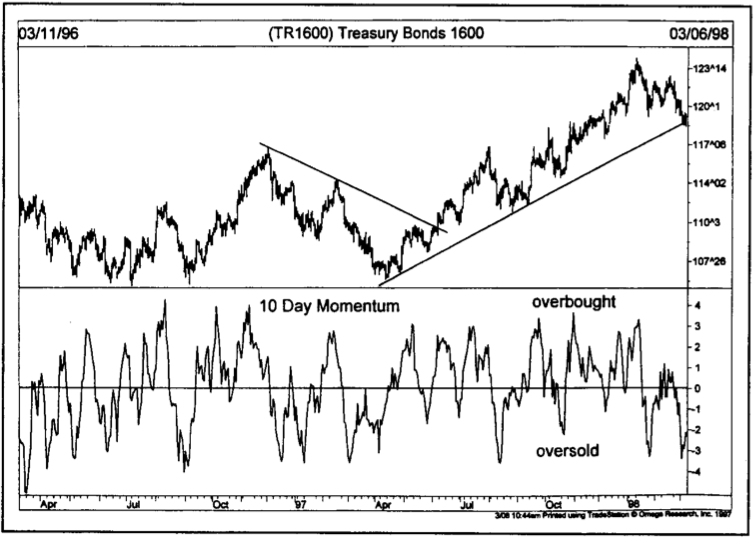
\includegraphics[width=0.8\textwidth]{graphics/fingrundlagen/momentum.png}
	\caption[10-Tage Momentum]{10-Tage Momentum, der �berkauft- und �berverkauft-Level anzeigt. \cite{murphy-technische}}
	\label{fig:momentum}
\end{figure}

%%%%%%%%%%%%%%%%%%%%%%%%%%%%%%%%%%%%%%%
\subsubsection{Relative Strength Indicator} \label{subsubsection:rsi}

Der \gls{rsi} gibt �hnliche Informationen wie das Momentum, schafft aber Abhilfe bei einigen Schwachstellen. Beispielsweise gibt es beim Momentum keine maximale Unter- und Obergrenze, wodurch es schwierig ist festzustellen, ob es sich momentan um eine Extremsituation handelt oder nicht. Der \gls{rsi} bewegt sich hingegen immer zwischen 0 und 100.
Eine wesentlich schwerwiegendere Schwachstelle des Momentums ist aber seine absolute Abh�ngigkeit von dem Kurs vor genau $n$ Zeitperioden. Sollte der Kurs zu der Zeit ein Hoch oder Tief erreicht haben, hat dies Auswirkungen auf das aktuelle Momentum, selbst wenn sich der aktuelle Kurs gar nicht oder nur kaum ver�ndert.\\

Der \gls{rsi} wird aus dem Durchschnitt der Schlusskurse von $n$ Tagen mit steigenden Kursen berechnet, dividiert durch den Durchschnitt der Schlusskurse von $n$ Tagen mit fallenden Kursen.\\

\begin{equation}
	\label{RS Up}
	RS_{Up} = \frac{\sum\limits_{i=0}^{n-1}{max(P_{t-i} - P_{t-i-1} ; 0)}}{n}
\end{equation}

\begin{equation}
	\label{RS Down}
	RS_{Down} = \frac{-\sum\limits_{i=0}^{n-1}{min(P_{t-i} - P_{t-i-1} ; 0)}}{n}
\end{equation}

Damit der \gls{rsi} immer zwischen 0 und 100 schwankt, kann nicht einfach $RS_{Up} / RS_{Down}$ berechnet werden, sondern es wird eine Normalisierung vorgenommen, die nichts an dem Aussehen
der \gls{rsi}-Kurve ver�ndert, sondern nur am Wertebereich.

\begin{equation}
	\label{RSI}
	RSI = \frac{RS_{Up}}{RS_{Up} + RS_{Down}}
\end{equation}

Der Erfinder sah urspr�nglich eine Zeitperiode von $n = 14$ Tagen vor, wobei aber f�r unterschiedliche Volatilit�t auch andere Parameter gew�hlt werden k�nnen. Interessant ist der \gls{rsi}, wenn er im Vorhinein festgelegte Level �berschreitet. Diese sind standardm��ig bei 70 und 30 f�r die �berkauft- und �berverkauft-Level, k�nnen aber beispielsweise als Anpassung f�r Bullenm�rkte auf 80 oder f�r B�renm�rkte auf 20 festgelegt werden.\cite{elder_living}

\begin{figure}
	\centering
		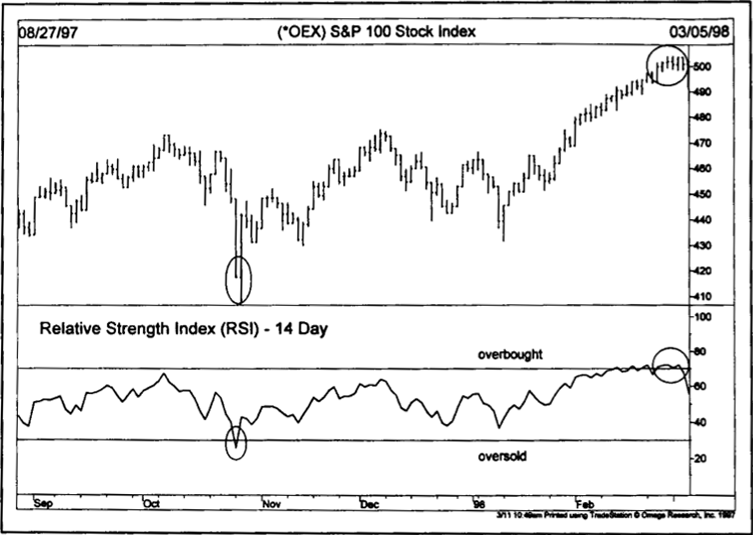
\includegraphics[width=0.8\textwidth]{graphics/fingrundlagen/rsi.png}
	\caption[14-Tage RSI]{14-Tage RSI am Beispiel des S\&P 100 \cite{murphy-technische}}
	\label{fig:rsi}
\end{figure}

%%%%%%%%%%%%%%%%%%%%%%%%%%%%%%%%%%%%%%%
\subsubsection{Prozentb�nder}

Prozentb�nder sind eine andere M�glichkeit, Nachhaltigkeit bzw. �berkauft- oder �berverkauft-Level festzustellen. Dazu wird ein \gls{ma} um einen festgelegten Prozentwert nach unten und oben verschoben, so dass ein Kanal bzw. ein Band entsteht, in dem der Kurs die meiste Zeit verl�uft. Wenn der Kurs �ber dem oberen Band notiert, wird dieser meist als �berkauft angesehen, da er im Vergleich zum Durchschnitt sehr schnell gestiegen ist. Um wie viel Prozent die B�nder nach oben und unten verschoben werden, h�ngt von der L�nge des \gls{ma} und somit dem Tradingzeitraum ab. Oft gebraucht werden 3\%-B�nder und eine 21-Tage-Linie oder 10\%-B�nder mit einem 40-Wochen-\gls{ma}.

%%%%%%%%%%%%%%%%%%%%%%%%%%%%%%%%%%%%%%%
\subsubsection{Bollinger B�nder}

Die Bollinger-B�nder, entwickelt von John Bollinger, sind ein �hnlicher Indikator wie die Prozentb�nder. Es wird ebenso ein Bereich oberhalb und unterhalb des \gls{ma} aufgespannt, aber anstatt ihn einfach um einen fixen Prozentwert zu verschieben, wird die Durchschnittslinie um die \emph{Doppelte Standardabweichung}, die meist auf L�nge des \gls{ma} berechnet wird, nach oben und nach unten verschoben.\\

Dabei dienen die B�nder meist als Kursziele, so dass beim Ansteigen des Kurses vom unteren Bollinger-Band das obere als Ziel angenommen wird. Diese Strategie wird auch als "`Fading"' bezeichnet und ist nur in Seitw�rtsphasen gewinnbringend, da der Preis w�hrend starken Trends lange Zeit entlang dem oberen oder unteren Rand des Bandes verlaufen kann. Die Breite der B�nder zeigt die Volatilit�t des Kurses an, da bei geringer Volatilit�t die Standardabweichung ebenfalls sinkt, ergo werden die B�nder schm�ler. Verschm�lern sich die B�nder in relativ kurzer Zeit, kann meist mit einem Ausbruch und einsetzendem Trend gerechnet werden. Bollinger B�nder k�nnen insgesamt sehr vielseitig eingesetzt werden, nicht nur in Seitw�rtsphasen, es existieren auch unterschiedliche Interpretations-Varianten.

\begin{figure}
	\centering
		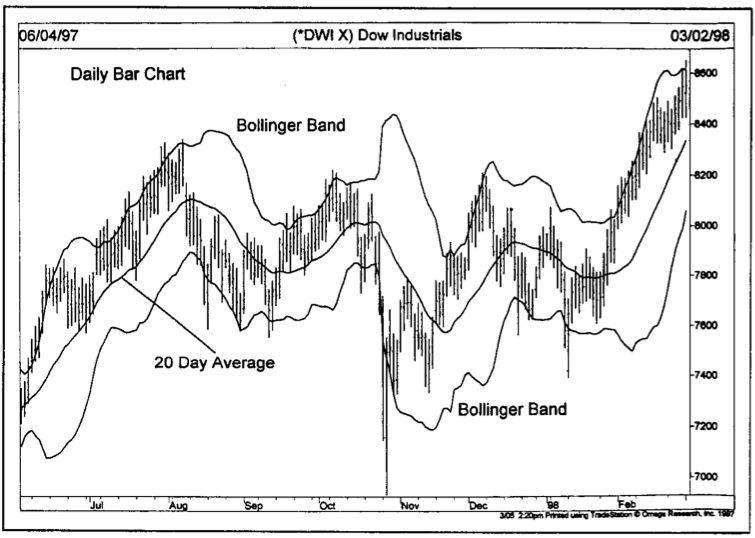
\includegraphics[width=0.8\textwidth]{graphics/fingrundlagen/bollinger.png}
	\caption[20-Tage Bollinger B�nder]{20-Tage Bollinger B�nder mit doppelter Standardabweichung am Beispiel des Dow Jones \cite{murphy-technische}}
	\label{fig:bollinger}
\end{figure}

%%%%%%%%%%%%%%%%%%%%%%%%%%%%%%%%%%%%%%%
\subsubsection{Pivot Points}

Pivot Points sind eine sehr h�ufig genutzte Variante zur Berechnung von horizontalen Support- und Resistance-Leveln. Dazu werden jeweils f�r eine Periode die Preisbewegungen der vorherigen Periode als Berechnungsgrundlage herangezogen. Als erstes wird der Typical Price (TP) der letzten Periode wie folgt berechnet.

\begin{equation}
TP = \frac{High+Low+Close}{3}
\end{equation}

Dieser wird als auch als Haupt-Pivot-Point bezeichnet, da von ihm ausgehend alle Unterst�tzungs- und Widerstandslevel festgelegt werden. Zur Berechnung verwendet werden immer die Daten aus der letzten Periode. Es werden zwei Level sowohl von Support- ($SL_1$ und $SL_2$) als auch von Resistance-Level ($RL_1$ und $RL_2$) berechnet, die je nach Marktsituation f�r unterschiedliche Zwecke ausgew�hlt werden k�nnen.

\begin{equation}
SL_1 = 2*TP - High
\end{equation} 

\begin{equation}
SL_2 = TP - (High - Low)
\end{equation} 

\begin{equation}
RL_1 = 2*TP - Low
\end{equation} 

\begin{equation}
RL_2 = TP + (High - Low)
\end{equation} 

\cite{tradimo_pivot_points}
% !TEX root = ../../Noctua_Diplomarbeit.tex

\subsection{Handelsstrategien mit MAs} \label{subsection:mastrategie}

Eine simples Tradingmodell basiert auf einer einfachen �berkreuzung eines \gls{ma} �ber den Preis. Es wird dabei angenommen, dass ein Aufw�rtstrend eingesetzt hat, wenn der Preis �ber den \gls{ma} steigt, da der Kurs begonnen hat, schneller als der Durchschnitt zu steigen. Umgekehrt wird angenommen, dass bei einem Abfall des Kurses unter den \gls{ma} ein Abw�rtstrend folgt und daher wird ein Short-Signal generiert. Eine zus�tzliche Sicherheit ist gegeben, wenn der \gls{ma} selbst in die erwartete Kursrichtung dreht. (siehe Abbildung \ref{fig:double_cross})

\begin{figure}
	\centering
		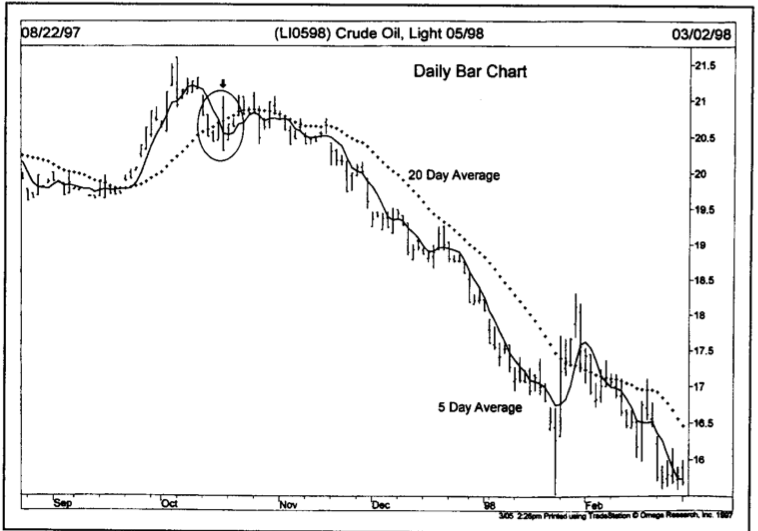
\includegraphics[width=0.8\textwidth]{graphics/fingrundlagen/double_cross.png}
	\caption[5,20 Double Cross Trading-System]{5,20 Double Cross Trading-System \cite{murphy-technische}}
	\label{fig:double_cross}
\end{figure}

Dieser simple Algorithmus hat einige Nachteile. Es wird zu jedem Zeitpunkt ein Signal gegeben, was bedeutet, dass immer entweder eine Long- oder eine Short-Position gehalten wird. Au�erdem verliert diese Strategie bei langen \glspl{ma} nach der Trendumkehr wieder viel vom Gewinn, da das Gegensignal erst sp�t generiert wird. Kurze \glspl{ma} erzeugen im Gegensatz dazu oft Fehlsignale.\\

Eine h�ufiger verwendete Variante zur Signalgenerierung mit \glspl{ma} wird \emph{Double Crossover Method} genannt. Dabei kommen zwei unterschiedlich lange \glspl{ma} zum Einsatz, wobei ein Signal erzeugt wird, wenn sich beide schneiden. Kreuzt der kurze \gls{ma} den l�ngeren, entsteht ein Kaufsignal, auch \emph{Golden Cross} genannt, und vice versa. Diese Variante erzeugt weniger Fehlsignale als die direkte Verwendung des Preises, hinkt dem Markt daf�r aber auch st�rker hinterher. Die L�nge der Durchschnitte h�ngt wie immer sowohl vom Handelszeitraum und der gew�nschten Signalanzahl als auch vom Markt ab.

Dieses System kann noch um einen weiteren \gls{ma} erweitert werden. Der Einsatz dreier Durchschnitte, oder \emph{Triple Crossover Method}, verfeinert die Signalgenerierung nochmals. Ein beginnender Aufw�rtstrend ist dann vorhanden, wenn der kurze \gls{ma} �ber dem mittleren liegt. Ein vollst�ndiges Kaufsignal entsteht, sobald der kurze �ber dem mittleren, und jener wiederum �ber dem langen \gls{ma} notiert. Eine umgekehrte Anordnung ist als Verkaufssignal anzusehen. Auf diese Art kann beispielsweise bei unklaren Signalen eine Neutralstellung (i.e. keine Aktien im Portfolio) eingenommen werden oder die Market-Exposure (i.e. Anzahl der Aktien) reduziert werden (siehe Abbildung \ref{fig:triple_cross}).
Normalerweise werden f�r solche Systeme \glspl{sma} verwendet, wobei aber besonders bei einem Double Cross\-over System auch die Anwendung eines \gls{ema},  \gls{dema} oder sogar \gls{tema} m�glich ist.

\begin{figure}
	\centering
		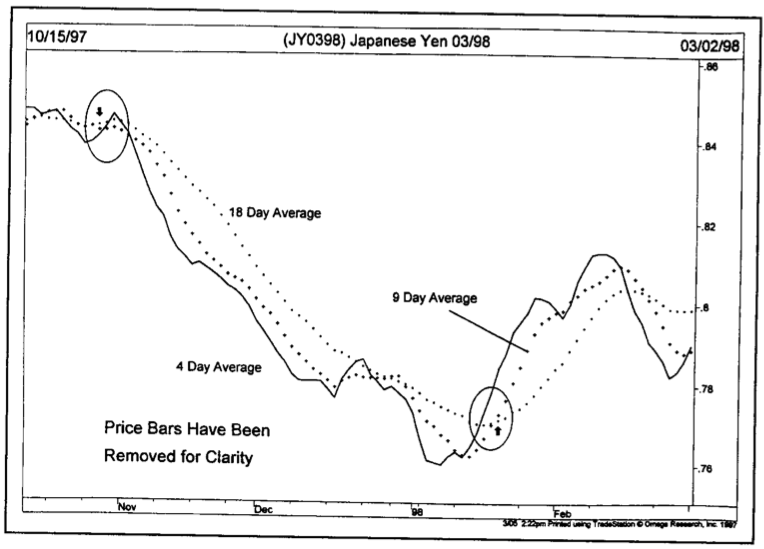
\includegraphics[width=0.8\textwidth]{graphics/fingrundlagen/triple_cross.png}
	\caption[4,9,18 Triple Cross Trading-System]{4,9,18 Triple Cross Trading-System \cite{murphy-technische}}
	\label{fig:triple_cross}
\end{figure}

\subsection{Fading-Strategie mit Bollinger B�ndern} \label{subsection:fading}

Seitw�rtsphasen zeichnen sich dadurch aus, dass der Preis mit einer gewissen Schwankungsbreite tendenziell weder steigt noch sinkt. Bollinger B�nder sind hervorragend daf�r geeignet, diese Schwankungsbreite statistisch abzubilden, da sie um ein Vielfaches der Standardabweichung (normalerweise der doppelten) des Durchschnitts nach oben und unten versetzt liegen. Um in dieser Situation Gewinn zu erzielen, w�re es daher vorteilhaft, dann zu kaufen, wenn der Preis nahe dem unteren Bollinger Band nach oben dreht und umgekehrt, wenn der Preis nahe dem oberen Bollinger Band nach unten dreht, zu verkaufen --- kurz gesagt, tief kaufen und hoch verkaufen. In l�ngeren Seitw�rtsphasen l�sst sich mit dieser Strategie gut ein Gewinn erzielen. Wenn die Bewegung jedoch recht schnell wieder einen Trend ausformt, muss dies schnell erkannt werden, um nicht zu viel des bereits erzielten Gewinns wieder zu verlieren. Anzeichen f�r einen einsetzenden Trend k�nnen z.B. kontrahierende Bollinger B�nder oder ein niedriger ADX-Wert sein.

% Alle Indikatoren beschreiben
% Quellen recherchieren
% Formel, wo m�glich
% Interpretation

\section{.NET-Framework}

% Was ist .NET
\subsection{Allgemein}

.NET ist ein Framework der Firma Microsoft, das eine Vielfalt an Sprachbibliotheken f�r eine gro�e Palette an Programmiersprachen zur Verf�gung stellt. Fr�her arbeiteten alle Programmiersprachen von Microsoft, wie bspw. C++, mit der WinAPI-32. Nun wurde dieses \gls{api} mit .NET durch ein sprachenunabh�ngiges, weitaus umfangreicheres Framework ersetzt. \cite{visualcsharp}\\
\\
Insgesamt wird die Nutzung des .NET-Frameworks von �ber 30 Programmiersprachen unterst�tzt. Die Richtlinien die eine Sprache einhalten muss, um als .NET-konform angesehen werden zu k�nnen, sind von Microsoft als \gls{cls} definiert worden. Zu den ber�hmtesten Vertretern solcher Sprachen Z�hlen C\#, F\#, Visual Basic .NET (VB.NET) und C++. \cite{visualcsharp}\\
\\
Zu den wichtigsten Features des .NET-Frameworks z�hlen die folgenden:
\begin{itemize}
\item \textbf{Objektorientierung} \\
	Das .NET-Framework ist zu 100\% objektbasiert. Das bedeutet, jegliche Elemente, sogar einfache Datentypen wie bspw. Integer, lassen sich auf Objekte zur�ckf�hren. Ja sogar die internen Zugriffe des Frameworks auf das darunterliegende Betriebssystem sind in Klassen gekapselt.
\item \textbf{Plattformunabh�ngigkeit} \\
	Anwendungen, die das .NET-Framework benutzen, werden �hnlich der \gls{jvm} erst zur Laufzeit in Maschinencode umgewandelt. Weiters ist die Spezifikation der von Microsoft benutzten Laufzeitumgebung, der sog. \gls{clr}, offen zug�nglich. Dadurch verlangt die Nutzung von .NET-Anwendungen also eine solche Umgebung, diese kann allerdings auch auf Plattformen portiert werden, die nicht Windows hei�en. So gibt es neben der propriet�ren Windows-Implementierung des .NET-Frameworks von Microsoft bspw. auch das \inline{Mono}-Projekt, mit dem .NET bereits erfolgreich auf Linux portiert werden konnte.
\item \textbf{Sprachenunabh�ngigkeit} \\
	Alle Komponenten des .NET-Frameworks k�nnen von jeder unterst�tzten Sprache problemlos verwendet werden. Das .NET-Framwork erm�glicht aber auch die Nutzung aller, in einer .NET-konformen Programmiersprache geschriebener Komponenten, in jeder anderen .NET-konformen Programmiersprache. So k�nnen zum Beispiel alle in C\# 2010 geschriebenen Klassen auch in F\# oder VB.NET genutzt und sogar abgeleitet werden.
\item \textbf{Speicherverwaltung} \\
	Die explizite Freigabe von nicht mehr ben�tigtem Speicher hat in der Vergangenheit schon zu vielen Problemen gef�hrt. Daf�r wurde mit dem .NET-Framework ein \inline{Garbage Collector} eingef�hrt, der dem Programmierer diese Aufgabe automatisch abnimmt. 
\item \textbf{Weitergabe} \\
	Auch die Weitergabe konnte deutlich vereinfacht werden. So k�nnen auf .NET basierende Sprachen einfach in eine .EXE- oder .\gls{dll}-Datei kompiliert und von jedem beliebigen Ordner aus ausgef�hrt werden. Eine .EXE-Datei ist dabei eine direkt ausf�hrbare Datei, deren Code bereits in einzelne Bytes umgewandelt wurde. \gls{dll}-Bibliotheken werden im folgenden Punkt erl�utert. \cite{visualcsharp}
\end{itemize}
% Was sind DLLs
% !TEX root = ../../Noctua_Diplomarbeit.tex

\subsection{Dynamic Link Library} \label{dll}

Alle .NET-Sprachen bieten die Funktionalit�t, Bibliotheksprojekte zu entwickeln. Normalerweise werden ausf�hrbare Programme entwickelt, w�hrend bei einem \gls{dll}-Projekt oder einer Bibliotheksanwendung nur eine Funktionalit�t implementiert werden muss. \cite{dllmsdn1}\\ \\
Eine DLL enth�lt Code und Daten. Man kann diese von mehreren Programmen gleichzeitig verwenden. Ihre Funktionalit�t ist allerdings nicht begrenzt, das bedeutet man kann mit ihnen genau die gleichen Ergebnisse erzielen, wie mit einer ausf�hrbaren Software, allerdings agiert eine \gls{dll} nicht von alleine. \\ \\
Prinzipiell werden \gls{dll}s programmiert um eine Software in unterschiedliche Komponenten (oder auch Modulen) zu trennen. Der Vorteil bei der Verwendung von \gls{dll}s ist die Einbindung in ein bestehendes Softwarekonstrukt zur Laufzeit, dass erh�ht die Erweiterbarkeit und Skalierbarkeit von Softwareprodukten. \cite{dllmsdn2} \\ \\
Bei einem Software-Update-Vorgang k�nnen beispielsweise nur die ver�nderten Komponenten vertauscht werden. Ein erneutes Installieren der Software ist somit nicht n�tig und kann vermieden werden. Im abstrakteren Geschehen bedeutet das, dass der Programmkern eine Ver�nderung der Funktionen nicht bemerkt und auch kein Teil der Erweiterung oder der Fehlerbehebung sein muss. Achtet man darauf komplexere Berechnungen in auswechselbaren Komponenten zu benutzen und die Komplexit�t des Kernprodukts gering zu halten, kann man ein Softwareprodukt leichter warten und weiterentwickeln. \cite{dllmsdn1}
\subsubsection{DLL-Typen}
Es gibt zwei M�glichkeiten die Funktionen einer DLL aufzurufen:
\begin{itemize}
	\item Load-Time Dynamic Linking
	\item Run-Time Dynamic Linking
\end{itemize}
Beim Load-Time Dynamic Linking wird bereits zur Kompilierzeit ein explizites Interface bereitgestellt, um die bereitgestellten Methoden explizit aufrufen zu k�nnen.\\ \\
Das Run-Time Dynamic Linking verwendet dynamische Methodenaufrufe, das bedeutet das auch beim Kompiliervorgang noch nicht klar ist welche Methoden die DLL bereitstellt. Die \gls{dll}s wird erst w�hrend der Laufzeit in die Software eingebunden. \cite{dllmsdn2}

\section{C\#-Grundlagen}

% Was ist C# (Microsoft)
% objektorientiert
\subsection{Allgemein}

Die Programmiersprache C\# wurde von der Firma Microsoft entwickelt und gilt als einer der wichtigsten Sprachen, die das .NET-Framework benutzen. C\# ist eine objektorientierte Programmiersprache mit einer fundamentalen Sprachsyntax. Mit diesen Eigenschaften eignet sie sich auch perfekt f�r die Nutzung von .NET. \cite{visualcsharp}\\
\\
Die Sprachsyntax von C\# ist der von Java sehr �hnlich. C\# wurde erstmals mit dem Ziel entwickelt, eine bessere, funktionsreichere Sprache zu entwickeln, die Java abl�sen k�nnte, trotzdem allerdings dessen Vorteile nutzt. Auch die allgemeine Struktur einer Klasse sowie der Aufbau simpler Anweisungen (if, for, while, etc.) sind quasi ident zu ihren �quivalenten in Java. \cite{visualcsharp}\\
\\
Eine C\#-Anwendung kann grunds�tzlich als Konsolenanwendung oder mit einer graphischen Oberfl�che (\gls{gui}) ausgef�hrt werden. Zur Realisierung einer solchen \gls{gui} werden ebenfalls mehrere Mechanismen zur Verf�hung gestellt. Zum einen gibt es die mittlerweile veraltete direkte M�glichkeit der Realisierung mit WinForms, einer API, die direkt in die Sprache integriert ist. Zum anderen hat Microsoft die \gls{wpf} entwickelt, die im folgenden Abschnitt \ref{wpf} genauer erl�utert wird. \cite{visualcsharp} \\
\\
Im folgenden sollen nun alle wichtigen Technologien der Sprache C\# beschrieben werden, die im Zuge dieses Projektes zum Einsatz gekommen sind.
% WPF
	% MVVM
	% XAML-GUI
	% GUI-Bindung
\subsection{Windows Presentation Foundation} \label{wpf}

Mit Version 3.0 des .NET-Frameworks wurde wie bereits erw�hnt zus�tzlich zur altbew�hrten WinForms-Variante, eine neue Variante integriert um Benutzeroberfl�chen einfach zu implementieren. Diese hei�t \gls{wpf}. \cite{visualcsharp}\\
\\
Das wichtigste Merkmal von \gls{wpf} gegen�ber anderen Methoden zur \gls{gui}-Erstellung ist, dass bei \gls{wpf} die Programmlogik nach strengsten Richtlinien von der Beschreibung der Oberfl�che trennt. Diese Beschreibung der Oberfl�che erfolgt mittels einer speziellen Version der normalen \gls{xml}, der \gls{xaml}. Mit dieser Sprache werden alle \gls{gui}-Komponenten, erzeugt und in die entsprechende Position gebracht. Bei \gls{wpf} wird allerdings trotzdem auch eine \gls{api} f�r den Zugriff auf \gls{xaml}-\gls{gui}-Komponenten innerhalb der Programmlogik bereit gestellt. Bei der Erstellung eines \gls{wpf}-Projektes, bekommt man automatisch ein MainWindow.xaml-File. Ein solches \gls{xaml}-File das lediglich einen Button als \gls{gui} anzeigt, w�rde nun in etwa so aussehen: \cite{visualcsharp}\\
\\
\begin{verbatim}
<Window x:Class="Wpf1Application1.MainWindow"
    xmlns="http://schemas.microsoft.com/winfx/2006/xaml/presentation"
    xmlns:x="http://schemas.microsoft.com/winfx/2006/xaml"
    Title="MainWindow" Height="350" Width="525">
    <Grid>
    	<Button Name="button1">Button</Button>
    <\Grid>
</Window>
\end{verbatim}

Hierbei werden zuerst die n�tigen von Microsoft definierten \gls{xaml}-Namespaces angegeben. Anschlie�end werden ein Titel (der ganz oben im Fenster angezeigt wird) und die Gr��e des Fensters angegeben, dass sp�ter unseren Button beinhalten soll. Danach wird ein einfaches Grid-Layout mit einem Button mit dem Text "Button" gezeichnet. Ab Microsoft Visual Studio 2008, wird auch ein \gls{wpf}-\gls{gui}-Builder bei der Installation mitgegeben, mit dem man diese \gls{xaml}-Dateien einfach mit graphischer Oberfl�che erstellen kann. \cite{visualcsharp}\\
\\
Zu der MainWindow.xaml-Datei wird auch noch eine weitere Datei mit dem Namen MainWindow.xaml.cs erstellt. Diese wird auch als \textit{Code-Behind}-Datei bezeichnet und beinhaltet den Teil der Programmlogik der direkt mit der graphischen Oberfl�che verkn�pft ist. M�chte man also bspw. die Logik implementieren, die beschreibt was bei einem Klick auf den Button passiert, m�sste man dies in eben dieser MainWindow.xaml.cs-Datei durchf�hren. \cite{visualcsharp}

\subsection{MVVM}
Als \gls{mvvm} wird ein Entwicklungsmuster (Design-Pattern) verstanden, dass sehr oft in Verbindung mit der Implementierung von \gls{wpf}-Oberfl�chen eingesetzt wird. Dabei werden die einzelnen Aufgaben einer Anwendung mit graphischer Oberfl�che in drei Teile aufgeteilt. Es gibt nun ein View, ein Model und ein ViewModel. Deren Interaktion kann in der Abbildung \ref{fig:mvvm} sehr sch�n nachvollzogen werden. \cite{msdn-mvvm}\\

\begin{figure}[h]
	\centering
		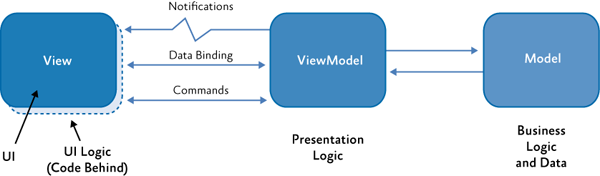
\includegraphics[width=0.90\textwidth]{graphics/grundlagen/mvvm.png}
	\caption{Aufbau von \gls{mvvm}}
	\label{fig:mvvm}
\end{figure}

Zuerst gibt es da also den View-Teil. Der View beschreibt das Aussehen der \gls{gui}. Im Optimalfall befindet sich um View ausschlie�lich ein Konstruktor mit einem Methodenaufruf InitializeComponents(), der die \gls{gui} �ber das \gls{xaml}-File aufbaut. Sollen allerdings komplexere graphisch aufwendigere Elemente oder Animationen in der grafischen Oberfl�che gezeichnet werden, kann diese Logik im View-Teil implementiert werden. Im View sollte allerdings nie Logik programmiert werden die man einem Unit-Testing unterziehen muss.\\ Wie der Abbildung \ref{fig:mvvm} entnommen werden kann, kommunziert der View nicht direkt, sondern ausschlie�lich �ber Commands, Notifications oder Data Binding mit dem ViewModel. Auf Commands wird hier nicht n�her eingegangen, Data Binding und Notifications k�nnen allerdings im folgenden Abschnitt \ref{databinding} gefunden werden. \cite{msdn-mvvm}\\
\\
Der ViewModel-Teil kapselt nun die Presentationslogik und die von der \gls{gui} ben�tigten Daten. Das ViewModel hat keinen direkten Zugriff auf den View und wei�t daher nichts �ber dessen Implementierung. Das ViewModel kann bspw. �ber die Verwaltung von Daten, die mittels Data Binding an den View weitergegeben werden mit diesem kommunizieren. Nebenbei bemerkt, m�ssen alle Daten die �ber Data Binding an den View weitergegeben werden sollen ausschlie�lich im ViewModel gespeichert werden. Das ViewModel beschreibt also welche Funktionalit�t die \gls{gui} anbieten soll und das View, wie diese angezeigt wird. Das ViewModel fungiert au�erdem quasi als Mittelmann zwischen dem View und dem Model und kann dabei bspw. noch die Daten aus dem Model so vereinfachen, dass der View diese leichter verarbeiten kann. \cite{msdn-mvvm}\\
\\
Das Model ist nun die eigentliche Gesch�fts- oder Programmlogik und die damit verbundenen allgemeinen Daten. Hierbei handelt es sich um eine ganz normale Gesch�ftslogik wie in anderen Anwendungen auch, nur dass noch einmal speziell Wert darauf gelegt werden sollte die einzelnen Codest�cke nicht Task-spezifisch zu implementieren, um die einzelnen St�ck sp�ter m�glicherweise an anderen Stellen wiederverwenden zu k�nnen. Au�erdem besteht das Model entgegen dem View und dem Viewmodel meist aus vielen einzelnen Model-Klassen, die alle mit dem selben ViewModel kommunizieren. M�chte das Model auch mit dem View interagieren gibt es auch hier die M�glichkeit Notifications zu benutzen.\cite{msdn-mvvm}

\subsection{Data Binding} \label{databinding}

Das Data Binding (auch: Datenbindung) erm�glicht \gls{gui}-Komponenten den Zugriff auf Daten, die sie anzeigen k�nnen. In WinForms war die Datenbindung auch schon integriert, lediglich war man mit den damaligen Methoden auf wenige Controls beschr�nkt. Mit \gls{wpf} ist man dies nun nicht mehr. Daten k�nnen hiermit n�mlich direkt aus einer der folgenden Datenquellen entnommen werden \cite{visualcsharp}:

\begin{itemize}
	\item ViewModel
	\item Eigenschaften anderer Komponenten
	\item \gls{xml}-Datei
	\item Collections
	\item Datenbanken
	\item etc.
\end{itemize} \cite{visualcsharp}

Zur Nutzung von Data Binding sind nun zwei Klassen wichtig, DataContext und Binding. Der DataContext ist die Datenquelle von der die Daten bezogen werden sollen. Dieser DataContext ist au�erdem ein Attribut jedes \gls{gui}-Elements und muss gesetzt werden, damit Bindungen funktionieren. M�chte man nun den DataContext setzen sollte man aber aufpassen und ihn im �bergeordneten Container (z.B. dem MainWindow) setzen, denn davon profitieren alle untergeordneten Komponenten dieses Conatiners und der DataContext muss nict �berall gesetzt werden. Das Binding-Objekt beschreibt nun die Binung zwischen einer Datenquelle und einer bindenden Komponente. Das Binding wird meist im \gls{xaml}-Code geschrieben, es besteht allerdings selbstverst�ndlich auch die M�glichkeit sie innerhalb des C\#-Codes zu erzeugen. \cite{visualcsharp}\\
\\
Das einfachste Beispiel f�r eine Bindung k�nnte nun in etwa so aussehen:

\begin{verbatim}
<Window x:Class="Wpf1Application1.MainWindow"
    xmlns="http://schemas.microsoft.com/winfx/2006/xaml/presentation"
    xmlns:x="http://schemas.microsoft.com/winfx/2006/xaml"
    Title="MainWindow" Height="350" Width="525">
    <Window.DataContext>
    	<local:MainViewModel x:Name="mainViewModel" />
    </Window.DataContext>
    <StackPanel>
    	<TextBox Name="txtOben" Height="50" FontSize="16"></TextBox>
    	<TextBox Name="txtUnten" Height="50" Background="AliceBlue" FontSize="16">
    		<Binding ElementName="txtOben" Path="Text" />
    	</TextBox>
    </StackPanel>
</Window>
\end{verbatim} \cite{visualcsharp}

Zuerst wird hier der \textit{DataContext} auf das ViewModel gesetzt. Dies w�re hier zwar noch nicht notwendig, da keine Bindung auf ein Property aus dem ViewModel erfolgt, es zeigt allerdings die angesprochene Funktionsweise und wird im n�chsten Beispiel von Bedeutung sein. Danach werden zwei \textit{TextBoxen} erstellt von denen die Text-Variable der unteren eine Bindung auf die Text-Variable der oberen besitzt. Dadurch wird der Text der unteren \textit{TextBox} automatisch an den Text der oberen \textit{TextBox} angepasst, falls sich dieser �ndert. Eine Bindung in dieser Art k�nnte aber auch auf jedes andere Attribute der \textit{TextBoxen} (z.B. Gr��e, Schriftart, etc.) angewendet werden. Dazu m�sste lediglich der \textit{Path} der Bindung ge�ndert werden. \cite{visualcsharp}\\
\\
Eine etwas kompliziertere Bindung ist die auf ein Property aus dem ViewModel. Dazu muss man zuerst im ViewModel ein Property erzeugen und dessen setter-Methode f�r die Nutzung von Notifications implementieren. Das Property, das die Lieblingsfarbe einer Person speichert, k�nnte dann in etwa so aussehen \cite{msdn-mvvm}:

\begin{verbatim}
public class MyViewModel : INotifyPropertyChanged
{
    private string favoriteColor;
    public event PropertyChangedEventHandler PropertyChanged;
    ...
    public string FavoriteColor
    {
        get { return this.favoriteColor; }
        set
        {
            if (value != this.favoriteColor)
            {
                this.favoriteColor = value;
                if (this.PropertyChanged != null)
                {
                    this.PropertyChanged(this,
                          new PropertyChangedEventArgs("FavoriteColor"));
                }
            }
        }
    }
}
\end{verbatim} \cite{msdn-mvvm}

Hierbei wird einfach eine globale Variable (\textit{favoriteColor}) mit einem Property (\textit{FavoriteColor}) versehen, das die setter-Methode so implementiert hat, dass ein \textit{PropertyChangedEvent} gesendet wird, sobald der Wert der Lieblingsfarbe ge�ndert wird. Dies ist notwendig, wenn man das Property an ein \gls{gui}-Element binden will, da sich das \gls{gui}-Element, sonst im Falle einer �nderung der Lieblingsfarbe nicht aktualisieren w�rde. M�chte man dieses Property nun im \gls{xaml}-Code an ein \gls{gui}-Element binden, muss man lediglich das Folgende schreiben:

\begin{verbatim}
<Window x:Class="Wpf1Application1.MainWindow"
    xmlns="http://schemas.microsoft.com/winfx/2006/xaml/presentation"
    xmlns:x="http://schemas.microsoft.com/winfx/2006/xaml"
    Title="MainWindow" Height="350" Width="525">
    <Window.DataContext>
    	<local:MainViewModel x:Name="mainViewModel" />
    </Window.DataContext>
    <StackPanel>
    	<TextBox Name="favoriteColorTextBox" Height="50" FontSize="16">
    		<Binding Path="FavoriteColor" />
    	</TextBox>
    </StackPanel>
</Window>
\end{verbatim}

Diesmal ist die Definition des ViewModels als \textit{DataContext} notwendig. Aus diesem wird n�mlich einfach in der Bindung das \textit{FavoriteColor}-Property aufgerufen. Schon steht zu jeder Zeit die aktuelle Lieblingsfarbe aus dem ViewModel in der \textit{TextBox}.
% Charting-Library (.NET)
\lstset{style=sharpc}
\subsection{Microsoft Chart Controls} \label{charting}

Die Microsoft Charts Controls Library ist eine sehr umfangreiche Bibliothek, die es erm�glicht in WinForms-Anwendungen oder auf Webseiten mit ASP.NET Charts und Diagramme zu zeichnen. Die M�glichkeiten sind derma�en umfangreich, dass es im Folgenden nur Sinn macht, die Funktionen zu erl�utern, die f�r die Darstellung finanzieller Charts erheblich sind. Zu den Hauptfeatures z�hlen daher \cite{msdn-charting}:

\begin{itemize}
\item \textbf{Charttypen} \\
	Es werden 35 verschiedene Charttypen unterst�tzt, dabei alles von normalen Liniencharts bis zu Bar- und Candlestick-Charts zur Darstellung von Aktiendaten.
\item \textbf{Skalierbarkeit} \\
	Es k�nnen unendlich viele Daten, Chart-Areas (Bereiche innerhalb eines Charts), Bemerkungen (z.B. Pfeile), etc. innerhalb eines Charts angezeigt werden. Daher k�nnen bspw. Aktiendaten und deren \glspl{ma} in einer ChartArea angezeigt werden. Zus�tzlich k�nnte man eine weitere ChartArea erg�nzen um bspw. einen \gls{macd}-Verlauf direkt unter den Aktiendaten zu zeichnen.
\item \textbf{Daten} \\
	Es werden Unmengen an M�glichkeiten zur Verwaltung der Daten innerhalb eines Charts, wie z.B. Data Binding, zur Verf�gung gestellt. Au�erdem k�nnen die Daten des Charts exportiert, oder zum Speichern serialisiert werden. 
\item \textbf{Aussehen} \\
	Weiters k�nnen sowohl zweidimensionale als auch dreidimensionale Charts erstellt werden, die alle sehr simpel und sch�n dargestellt werden. Die k�nnen zudem auch zur Laufzeit noch weiter manipuliert werden und die WinForms-Version bietet sogar M�glichkeiten zum interaktiven Zoomen und Scrollen f�r den User. (Auf Webseiten mit ASP.NET werden keine interaktiven Funktionen f�r den Benutzer der Website angeboten.) 
\end{itemize} \cite{msdn-charting}

\subsubsection{Nutzung mit WPF} \label{winformshost}

Leider ist momentan noch keine Version f�r die Verwendung mit \gls{wpf} erh�ltlich, man kann diese Einschr�nkung allerdings umgehen indem man einen sog. \textit{WinFormsHost} erstellt. Dies ist ein \gls{wpf}-\gls{gui}-Element, das WinForms-Elemente so kapselt, dass sie in \gls{wpf} genutzt werden k�nnen. Dieses Element mit einem \textit{MSChart} kann so erstellt werden:

\begin{lstlisting}[label=MSChart in einer WinFormsHost-Umgebung,caption=MSChart in einer WinFormsHost-Umgebung]
<WindowsFormsHost Name="WfHost" Grid.Row="0">
	<MSChart:Chart x:Name="MyWinformChart">
	    <MSChart:Chart.ChartAreas>
	        <MSChart:ChartArea Name="MainArea"/>
	    </MSChart:Chart.ChartAreas>
	</MSChart:Chart>
</WindowsFormsHost>
\end{lstlisting}

Hier wurde au�er dem primitiven \textit{MSChart} auch gleich eine \textit{ChartArea} hinzugef�gt. Eine \textit{ChartArea} ist ein Bereich innerhalb des Charts (hier der gesamte Bereich des Charts), in dem eine Funktion gezeichnet werden kann. Damit dieses WinFormsHost-Element allerdings funktioniert m�ssen f�r das gesamte \textit{Window} noch folgende Namespaces erg�nzt werden (diese Assemblies m�ssen nat�rlich auch als Verweis zum Projekt hinzugef�gt werden):

\begin{lstlisting}[label=Namespaces f�r MSChart und WinFormsHost,caption=Namespaces f�r MSChart und WinFormsHost]
xmlns:wf="clr-namespace:System.Windows.Forms;assembly=System.Windows.Forms"
xmlns:MSChart="clr-namespace:System.Windows.Forms.DataVisualization.Charting;assembly=System.Windows.Forms.DataVisualization"
xmlns:wfi="clr-namespace:System.Windows.Forms.Integration;assembly=WindowsFormsIntegration"
\end{lstlisting}

\subsubsection{Darstellung einfacher Graphen}

Nachdem eine leere \textit{ChartArea}, in die ein Graph gezeichnet werden kann, bereits im \gls{xaml} erzeugt wurde, muss man im C\#-Code nur noch das \textit{Chart} suchen, in das gezeichnet werden soll und eine \textit{Series} erstellen. In diese Series werden dann die Daten eingespeist, die gezeichnet werden soll. Wenn man nun auch noch einen Typ f�r den Graphen konfiguriert wird dieser auch schon in der \textit{ChartArea} angezeigt. Um bspw. eine Sinusfunktion darzustellen m�sste man nun folgenden Code schreiben: \cite{msdn-charting}

\begin{lstlisting}[label=Erstellung einer Series,caption=Erstellung einer Series]
//Lookup des bereits im XAMl-Code definierten Charts
Chart chart = this.FindName("MyWinformChart") as Chart;

//Erstellen der Series
Series sinus = new Series("Sinus");

//Berechnung einer Sinuskurve und speichern der
//errechneten Daten in die Series
for (double i = 0; i <= 7.5; i += 0.2)
	sinus.Points.AddXY(i, Math.Sin(i));

//Definieren des Zeichentyps als normale Linie
sinus.ChartType = SeriesChartType.FastLine;
 
// Hinzufuegen des Graphs zum Chart
chart.Series.Add(sinus);
\end{lstlisting} \cite{mschart-grundlagen}

In diesem Beispiel wurde jeder Punkt des Sinus einzeln berechnet und zur \textit{Series} hinzugef�gt. Dies k�nnte man nat�rlich auch mit jeder anderen Datenquelle wie zum Beispiel einer Liste machen, in dem man jeden Wert einzeln hinzuf�gt. \cite{msdn-charting}

\subsubsection{Finanzielle Berechnungen} \label{finfor}

Die Microsoft Chart Controls Library bietet allerdings nicht nur M�glichkeiten zur einfachen Darstellung von Daten. Denn sie beinhaltet ein Framework aus �ber 50 veschiedenen statistischen und finanziellen Formeln zur automatischen Berechnung und Darstellung spezieller Werte. \cite{msdn-charting}\\
\\
Die wichtigsten Formeln in der \textit{FinancialFormula}-Sammlung der MS Chart Controls sind:

\begin{itemize}
\item Bollinger B�nder
\item \gls{cci}
\item diverse \glspl{ma}
\item \gls{macd}
\end{itemize} \cite{msdn-charting}

Im Code w�rde der Einsatz von \textit{FinancialFormula} so aussehen:

\begin{lstlisting} [label=Berechnung eines WMA mit FinancialFormula,caption=Berechnung eines WMA mit FinancialFormula]
chart.DataManipulator.FinancialFormula(FinancialFormula.WeightedMovingAverage, 90, "Data", "FinFor");
\end{lstlisting} \cite{msdn-charting}

Dieser Aufruf erzeugt einen \gls{ma} der L�nge 90. Dazu holt er sich die Daten aus der Series ''\textit{Data}'', berechnet den \gls{ma} und schreibt die errechneten Daten in die \textit{Series FinFor}. Damit diese Berechnung m�glich ist muss die \textit{Series FinFor} bereits zuvor erzeugt und die \textit{Series Data} ebenfalls bereits zuvor erzeugt auch wirklich mit Daten gef�llt sein. \cite{msdn-charting}
% C# Tuples
\lstset{style=sharpc}
\subsection{C\# Tupel}

Ein Tupel ist prinzipiell eine Ansammlung von Werten. Dabei kann es beliebig viele Werte mit verschiedenen Datentypen haben. Eben diese Anzahl und die dazugeh�rigen Datentypen m�ssen allerdings schon im Vorhinein festgelegt werden, wenn das Tupel erzeugt wird. Ein \inline{Tuple} in C\# k�nnte bspw. so aussehen \cite{cs-tuple}:

\begin{lstlisting} [label=Erstellung eines Tuples,caption=Erstellung eines Tuples]
Tuple<int, bool> tuple = new Tuple<int, bool>(1, true);
\end{lstlisting}

Dabei handelt es sich um ein sehr einfaches \inline{Tuple}, das lediglich einen Integer-Wert zu einem dazugeh�rigen Boolean-Wert speichert. Ein \inline{Tuple} ist eine Klasse, in der direkt Werte gespeichert werden. Deshalb muss er einen separaten Ort im Heap allokieren. \cite{cs-tuple} Dies bedeutet, dass bspw. ein Tupel mit zwei Werten in der Erstellung wesentlich l�nger ben�tigt als ein \inline{KeyValuePair}, es aber sp�ter in der Nutzung eine deutlich h�here Performance aufweist. \cite{tuple-performance} Au�erdem k�nnen durch diese Tatsache die Datentypen der Felder des Tupels nach dessen Erstellung absolut nicht mehr ge�ndert werden, was das \inline{Tuple} eigentlich mehr einer \inline{struct} �hneln l�sst. \cite{cs-tuple}\\
\\
In der Praxis werden selten einzelne Tupel verwendet. Es ist allerdings oft von Vorteil eine Liste aus Tupeln zu erzeugen, wenn man quasi eine \inline{Map} (bzw. ein \inline{Dictionary}) mit mehreren Werten oder anderen Datentypen ben�tigt. So k�nnen z.B. Aktienpreis-Bars als Tupel aus einem \inline{TimeStamp} und Feldern f�r Open, High, Low und Close realisiert werden. Daraus kann dann eine Liste erstellt werden, um die Bars ad�quat speichern zu k�nnen.
% Speichern
\lstset{style=sharpc}
\subsection{Bin�re Serialisierung} \label{Binaere-Serialisierung}

Objekte in .NET-Sprachen sind grunds�tzlich fl�chtig, dass bedeutet das sie nach der Beendung und einem anschlie�enden Neustart der Anwendung nicht mehr vorhanden sind. Oft ben�tigen Entwickler allerdings die Funktion, solche Objekte zu persistieren, sie also nach einem Neustart der Applikation weiterhin verf�gbar zu machen. Dies kann durch bin�re Serialisierung erreicht werden. Bei diesem Verfahren k�nnen �ber einen sog. \textit{BinaryFormatter} alle als \textit{Serializable} gekennzeichneten Objekte und deren aktueller Zustand, sprich all deren Variablenwerte, in bin�ren Code umgewandelt werden. Dieser bin�re Code k�nnte bspw. in einer persistenten Datei, einer Datenbank oder einer Anwendungskonfigurationsdatei (Siehe \ref{akd}) gespeichert werden. Weiters k�nnte dieser serialisierte Bin�rcode eines Objektes auch leicht �ber das Netzwerk �bertragen werden, ohne dass die einzelnen Softwarekomponenten auf dem Weg des Objekts auch dessen Definition (Klasse) kennen m�ssen. \cite{visualcsharp}

\subsubsection{Anwendung}

Neben der einfachen Serialisierung mit dem \textit{BinaryFormatter}, bietet das .NET-Framework auch einen \textit{SoapFormatter} und einen \textit{XmlSerializer}. Der \textit{SoapFormatter} �bertr�gt den aktuellen Zustand eines Objekts nicht in ein bin�res, sondern in ein \gls{soap}-Format. Dieses wird bei der �bertragung von Daten �ber das Netzwerk mittels einer \gls{soap}-Verbindung ben�tigt, um Objekte �bertragen zu k�nnen. Der \textit{XmlSerializer} �bertr�gt die Daten des betroffenen Objekts in ein \gls{xml}-Format, um es als \gls{xml}-Datei abspeichern und ggf. sp�ter wieder auslesen zu k�nnen. Im folgenden werde ich allerdings nur auf den wichtigsten, den \textit{BinaryFormatter}, eingehen, der Objekte einfach in ein bin�res Format �berf�hrt und auf einen Stream legt. Dazu m�ssen lediglich alle globalen Variablen bzw. deren Werte in Bin�rcode umgewandelt und gespeichert werden. Methodendefinitionen, etc., m�ssen dabei nicht serialisiert werden, da zur Deserialisierung und anschlie�enden Nutzung des Objekts die Klassendefinition des Objekts ohnehin vorhanden sein muss. Die Serialisierung funktioniert wie folgt \cite{visualcsharp}:

\begin{lstlisting}[label=Serialisierung mit einem BinaryFormatter,caption=Serialisierung mit einem BinaryFormatter]
BinaryFormatter bFormatter = new BinaryFormatter();
bFormatter.Serialize(stream, object);
\end{lstlisting}

Dazu wird also zuerst ein neuer \textit{BinaryFormatter} initialisiert und anschlie�end die \textit{Serialize}-Methode aufgerufen. Der \textit{Serialize}-Methode muss dabei zuerst ein Stream �bergeben werden. Bei diesem Stream wird es sich meist um einen \textit{FileStream} handeln, der das umgewandelte Objekt auch sofort in eine Datei schreibt. Es kann allerdings bspw. auch ein Kommunikationsstream oder jede andere m�gliche Art von Streams, die vom Objekt \textit{Stream} erbt, �bergeben werden. Als zweiter Parameter kann jedes m�gliche Objekt, dessen Klasse von \textit{Object} erbt und mit dem \textit{Serializable()}-Attribut gekennzeichnet ist, �bergeben werden. Es kann hier aber auch bspw. eine Liste �bergeben werden, sofern sowohl die Liste selbst als auch all ihre gespeicherten Elemente das \textit{Serializable()}-Attribut besitzen. \cite{visualcsharp}\\
\\
Eine Klasse kann wie folgt bei der Deklaration mit dem \textit{Serializable()}-Attribut gekennzeichnet werden \cite{visualcsharp}:

\begin{lstlisting}[label=Markierung einer Klasse als Serializable,caption=Markierung einer Klasse als Serializable]
[Serializable()]
class Klasse{
	...
}
\end{lstlisting}

Dies ist lediglich die Markierung der Klasse �ber ein sog. Markup-Interface. Dadurch wird der Compiler dar�ber informiert, dass Objekte dieser Klasse keinen au�ergew�hnlich heiklen Inhalt beinhalten und somit bedenkenlos serialisiert werden d�rfen. Fehlt dieses Attribut, so wird eine \textit{SerializationException} ausgel�st. \cite{visualcsharp}\\
\\
M�chte man ein bereits serialisiertes Objekt aus dem Bin�rcode wieder auslesen und als Objekt speichern, ben�tigt man ebenfalls die Klasse \textit{BinaryFormatter} und dessen \textit{Deserialize}-Methode. Dieser muss nur der Stream �bergeben werden, der sich ohnehin mit seinem internen Zeiger auf einer Position befindet. Mit dem Aufruf der \textit{Deserialize}-Methode wird ab der aktuellen Zeigerposition das n�chste serialisierte Objekt gesucht, zur�ck in ein normales Objekt umgewandelt und als \textit{Object} zur�ckgegeben. Damit dieses \textit{Object} wieder als das urspr�ngliche erkannt wird und mit der richtigen Klassendefinition verkn�pft wird, muss es zus�tzlich noch auf den gew�nschten Typ gecastet werden. \cite{visualcsharp}

\begin{lstlisting}[label=Deserialisierung mit einem BinaryFormatter,caption=Deserialisierung mit einem BinaryFormatter]
BinaryFormatter bFormatter = new BinaryFormatter();
Object object = (Object) bFormatter.Deserialize(stream);
\end{lstlisting}

\subsection{Konfigurationsdateien}

Das .NET-Framework unterst�tzt die Nutzung vieler verschiedener Konfigurationsdateien. Diese Konfigurationsdateien beinhalten grunds�tzlich einfach nur Daten, die zur Laufzeit von der Anwendung ausgelesen werden k�nnen. Dadurch kann bspw. das Laufzeitverhalten der Anwendung komplett ver�ndert werden oder einfach nur ein einfach verwalteter Datenspeicher eingerichtet werden. Es gibt Anwendungskonfigurationsdateien, Herausgeberrichtliniendateien und die Maschienenkonfigurationsdatei, die beim Start der Anwendung auch in dieser Reihenfolge aufgerufen werden. Im folgenden wird allerdings lediglich auf die Anwendungskonfigurationsdateien eingegangen.  \cite{visualcsharp}

\subsubsection{Anwendungskonfigurationsdateien} \label{akd}

Eine Anwendungskonfigurationsdatei ist f�r die Ausf�hrung einer Anwendung optional. Ist sie allerdings vorhanden, so dient sie zur Verwaltung und Sicherung der Stammdaten der gesamten Anwendung im \gls{xml}-Format. Diese Datei befindet sich immer im Stammverzeichnis der Anwendung und ihr Name setzt sich aus dem Namen der Anwendung und dem Suffix \textit{.config} zusammen. Meist wird sie dazu verwendet, den aktuellen Zustand einer Anwendung, das bedeutet alle zur Laufzeit gesetzten Variablen, zu sichern, um sie sp�ter im selben Zustand neu starten zu k�nnen. Dazu werden meist alle wichtigen Daten beim Beenden der Applikation in die Anwendungskonfigurationsdatei gespeichert und beim Start der Anwendung erneut aus dieser ausgelesen. \cite{visualcsharp}\\
\\
Innerhalb der \gls{xml}-Datei in der \textit{<configuration>}-Sektion werden zur Verwaltung dieser Stammdaten vier verschiedene Code-Sektionen angeboten. \cite{visualcsharp}

\begin{itemize}
\item \textit{<configSections>} \\
	Diese Sektion beschreibt lediglich das Ausma� der beiden untergeordneten Sektionen \textit{<applicationSettings>} und \textit{<userSettings>}.
\item \textit{<applicationSettings>} \\
	Diese Sektion speichert alle Stammdaten, die f�r die gesamte Anwendung (und jeden Benutzer) g�ltig sein sollen.
\item \textit{<userSettings>} \\
	Diese Sektion erlaubt die Definition und Sicherung von Stammdaten der Anwendung, die immer nur f�r einen einzigen Benutzer g�ltig sind. Dies ist besonders f�r benutzerspezifische Einstellungen unentbehrlich.
\item \textit{<appSettings>} \\
	Diese Sektion bietet grunds�tzlich die selben Funktionen wie die Sektion \textit{<applicationSettings>}, kann jedoch aus dem Code der laufenden Anwendung heraus editiert werden. \cite{visualcsharp}
\end{itemize}

Da die manuelle Erstellung einer solchen Anwendungskonfigurationsdatei sehr kompliziert w�re und mit einem sehr gro�en Aufwand verbunden ist, hat Microsoft eine unterst�tzte Erstellungshilfe mit graphischer Oberfl�che in seine Entwicklungsumgebung Visual Studio integriert. Dazu m�ssen nur die Project-Properties des entsprechenden Projekts ge�ffnet und hier der Tab "`Einstellungen"' gew�hlt werden. Dadurch kommt man zu der Oberfl�che aus Abbildung \ref{fig:akdErstellung}. \cite{visualcsharp}

\begin{figure}[h]
	\centering
		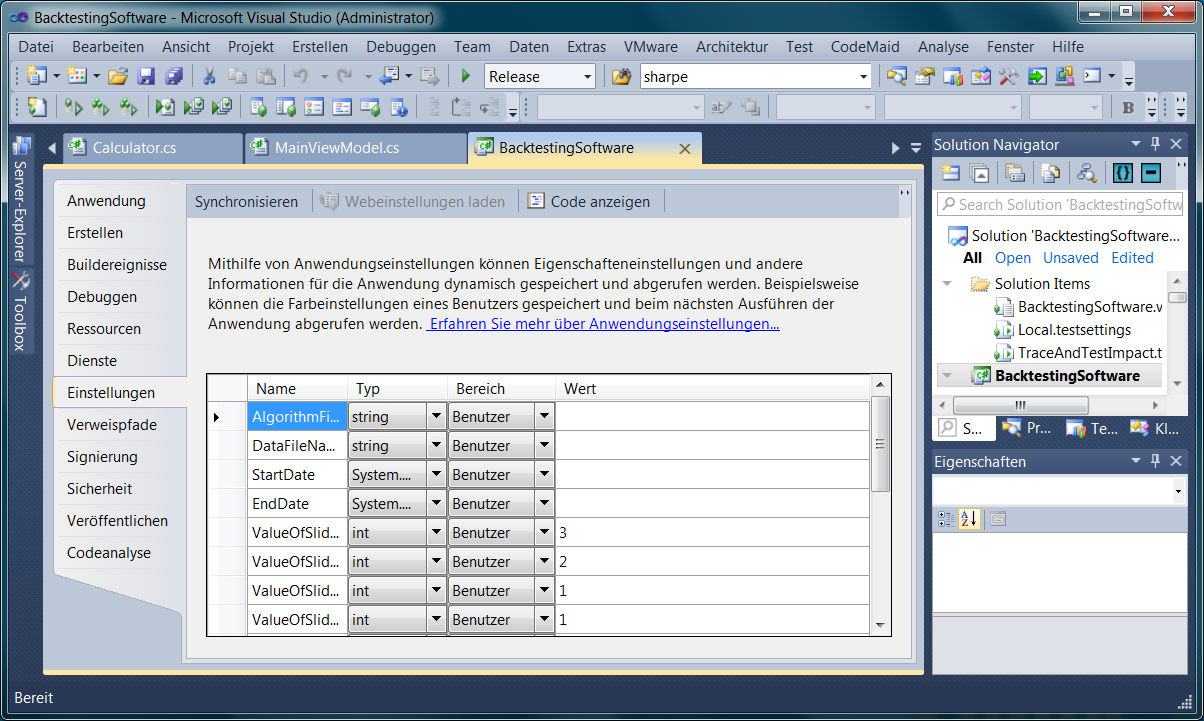
\includegraphics[width=0.90\textwidth]{graphics/grundlagen/akdErstellung.png}
	\caption{Erstellung einer Anwendungskonfigurationsdatei mit Hilfe von Microsoft Visual Studio}
	\label{fig:akdErstellung}
\end{figure}

Hier wurden schon einige Datens�tze hinzugef�gt. Wie man sehen kann, muss lediglich f�r jeden neuen Datensatz eine neue Zeile angelegt werden. Danach muss der Einstellung ein Name und ein Datentyp zugewiesen werden. Spezifische Datentypen bzw. eigens kreierte Objekte k�nnen nicht als Einstellung in der Anwendungskonfigurationsdatei definiert werden, sie k�nnen allerdings bspw. in serialisierter Form als String gespeichert werden. Nun m�ssen nur noch eine der zuvor beschriebenen Code-Sektionen als Bereich und ein Startwert, der nach der Erzeugung der \gls{xml}-Datei zu Anfang als Wert dieses Datensatzes gespeichert wird, definiert werden und schon kann der Datensatz im Programmcode benutzt werden. Das Lesen und Schreiben in ein solches File im Programmcode am Beispiel eines \textit{string}s f�r den Namen der Algorithmus-\gls{dll}-Datei funktioniert wie folgt \cite{visualcsharp}:

\begin{lstlisting}[label=Nutzung einer Anwendungskonfigurationsdatei,caption=Nutzung einer Anwendungskonfigurationsdatei]
string algorithmFileName = "algorithm.dll";
//Schreiben
Properties.Settings.Default.AlgorithmFileName = algorithmFileName;
//Lesen
string algorithmFileNameRestored = Properties.Settings.Default.AlgorithmFileName;
\end{lstlisting}

Zu den Default-Settings auf die in diesem Beispiel zugegriffen wird, k�nnen nat�rlich auch noch weitere Settings definiert werden. \cite{visualcsharp}
% LINQ
\lstset{style=sharpc}
\subsection{LINQ} \label{linq}

\gls{linq} stellt eine Spracherweiterung zu .NET dar, die mit dem .NET-Framework 3.5 und der Visual Studio Version 2008 hinzugef�hgt wurde. \gls{linq} erm�glicht es �ber ein neues Abstraktionsmodell aus vielen verschiedenen Datenquellen �ber die selbe Syntax Daten abzufragen. Unterst�tzt werden bspw. \gls{xml}-Dokumente, Datenbanktabellen, Excel-Tabellen, herk�mmliche Objekte oder Auflistungen von Objekten aller Art, und vieles mehr. \cite{visualcsharp}\\
\\
Da der Zugriff auf unterschiedliche Datenquellen intern allerdings durchaus unterschiedlich ablaufen muss, wurden von Microsoft mehrere \gls{linq}-Implementierungen in das .NET-Framework integriert. Diese werden Provider genannt und existieren zum Beispiel f�r folgende Datenquellen \cite{visualcsharp}:

\begin{itemize}
\item \textbf{\gls{linq} to Objects} \\
	Mit dieser Implementierung lassen sich Auflistungen und Objekte manipulieren, die untereinander auch in Beziehung gesetzt werden k�nnen. Sie stellt damit das Fundament aller\gls{linq}-Abfragen dar.
\item \textbf{\gls{linq} to \gls{xml}} \\
	Diese Implementierung nutzt das .NET sprachinterne Abfrage-Framework f�r den Zugriff auf \gls{xml} im Arbeitsspeicher.
\item \textbf{\gls{linq} to \gls{sql}} \\
	Hiermit kann auf Microsofts hauseigenes Datenbanksystem \gls{sql} Server 2005 und 2008 zugegriffen werden.
\end{itemize} \cite{visualcsharp}

\subsubsection{Aufbau einer LINQ-Anweisung}

Optisch sieht der Aufbau einer \gls{linq}-Anweisung, dem einer \gls{sql}-\textit{SELECT}-Anweisung sehr �hnlich. Eine Abfrage zur Ermittlung aller Personen mit Alter �ber 30 Jahren und der R�ckgabe derer Alter und Namen in einer Ergebnisliste, w�rde als \gls{linq}-Anweisung in etwa so aussehen \cite{visualcsharp}:

\begin{lstlisting}
var pers = from p in personen
		   where p.Alter > 30
		   select new { p.Name, p.Alter };
\end{lstlisting} \cite{visualcsharp}

Genau die selbe Funktion, nur mit einer anderen Formulierung w�rde auch die folgende Abfrage erf�llen \cite{visualcsharp}:

\begin{lstlisting}
var pers = personen
		  .Where( p => p.Alter > 30 )
		  .Select( p => new {p.Name, p.Alter });
\end{lstlisting} \cite{visualcsharp}

Dabei ist es v�llig egal, ob \textit{personen} das Ergebnis einer Datenbankabfrage oder eine Liste von \textit{Person}-Objekten ist, mit \gls{linq} muss man nur eine der beiden gezeigten Abfrage-Varianten benutzen.  Weiters erm�glicht die Nutzung von \gls{linq} auch viele zus�tzliche Optionen, die das Suchergebnis weiter verfeinern. Es gibt bspw. die \gls{sql}-�hnlichen Funktionen, wie \textit{GroupBy} und \textit{Join}, es gibt allerdings auch noch viele mehr. \cite{visualcsharp}

\subsubsection{Interne Funktionsweise von LINQ-Abfragen}

\gls{linq}-Abfragen machen oft Gebrauch vom Prinzip der \textit{Delegates}. \textit{Delegate} ist eine relativ alte Technologie, die in der Programmiersprache C schon unter dem Namen Funktionszeiger bekannt war. Ein \textit{Delegate} ist ein Typ, der auf eine Methode zeigt. Das Wort ''Delegate'' kommt von ''Delegierter'' und wurde gew�hlt, da ein \textit{Delegate} wirklich einen Methodenaufruf an eine bestimmte andere Methode weiter leitet. Dies wird innerhalb von \gls{linq}-Abfragen ben�tigt, um die vom User �bergebenen Bedingungen in die Logik der intern genutzten Methoden integrieren zu k�nnen. Der wohl am meisten in Kombination mit \gls{linq}-Abfragen genutzte \textit{Delegate} ist der folgende \cite{visualcsharp}:

\begin{lstlisting}
public delegate TResult Func<T, TResult>(T arg)
\end{lstlisting} \cite{visualcsharp}

Dieser wurde bspw. im oberen Beispiel verwendet, um die Bedingungen der \textit{Where}- (\textit{p => p.Alter > 30}) und der \textit{Select}-Abfrage (\textit{p => new {p.Name, p.Alter }}) an die \gls{linq}-Logik zu �bergeben. Beide dieser Bedingungen werden hier als Methodenaufrufe bzw. Zeiger auf Methodenaufrufe mit einem R�ckgabewert an die innere Logik der \gls{linq} �bergeben. Das \textit{T} in \textit{Func<T, TResult>} beschreibt einen generischen Datentypen mit dem innerhalb der Abfrage gearbeitet werden soll. Hier k�nnen alle existierenden primitiven Datentypen �bergeben werden und die Logik der \gls{linq} kann problemlos damit arbeiten. \textit{TResult} beschreibt ebenfalls einen generischen Datentypen. Allerdings den der vom angezeigten Methodenaufruf zur�ckgegeben wird. Intern ist die Abfragelogik der \gls{linq} damit so organisiert \cite{visualcsharp}:

\begin{lstlisting}
class Programm {
	static void Main(string[] args) {
		string[] arr = { "Peter", "Uwe", "Willi", "Udo" };
		GetShortNames(arr, name => name.Length < 4 );
		Console.ReadLine();
	}
	
	static void GetShortNames<T>(T[] names, Func<T, bool> getNames) {
		foreach (T name in names )
			if (getNames(name))
				Console.WriteLine(name);
	}
}
\end{lstlisting} \cite{visualcsharp}

In diesem Beispiel wird der Methode \textit{GetShortNames} ein \textit{Delegate} �bergeben, der angibt welche Namen der Namensliste ausgegeben werden soll. Hierbei h�tte in der \textit{Main}-Methode auch jede beliebige andere Bedingung, wie zum Beispiel die Abfrage, ob der erste Buchstabe des Namens ein ''P'' ist (\textit{GetShortNames(arr, name => name[0] == 'P');}) und es w�re genauso der entsprechende Name ''Peter'' ausgegeben worden, ohne dass die Methode ge�ndert werden musste. \cite{visualcsharp}

\clearpage
\section{F\#-Grundlagen}
\lstset{language=FSharp,caption={Descriptive Caption Text},label=DescriptiveLabel}
\section{F-Sharp Grundlagen}
F-Sharp (Visual F\# oder auch F\#,) ist eine, im Grunde gesehen, funktionale Programmiersprache, welche auf gro�e Datenmengen und schnelle Berechnungen optimiert ist. Die m�gliche Interoperabilit�t mit allen .NET-Sprachen macht die Sprache zu einer idealen Komponente eines Softwareprodukts. F-Sharp ist konzipiert um auf eine gro�e Menge an Daten zu wirken, dies wird mittels zus�tzlichen Methoden f�r Listen, Sequenzen und Arrays m�glich gemacht. \cite{fsharp}  \\
Der Begriff funktionale Programmiersprache beschreibt eine Programmiersprache die nur aus Funktionen besteht. Bei einer Funktion handelt es sich um eine Prozedur, die als Ziel eine Auswertung hat. Im Gegenzug dazu steht die imperative Programmierung, ein Programm, das in solch einer Sprache geschrieben ist, folgt den einzelnen Anweisungen des Quellcodes. \cite{programmingparadigms}\\
Durch die Anbindung an das .Net-Framework wird F-Sharp allerdings zu einer Multi-Paradigmen-Sprache. Es wird erm�glicht funktional, objektorientiert, aber auch imperativ arbeiten zu k�nnen. \cite{fsharp}\\
\begin{figure}[h]
	\centering
     
\includegraphics[scale=1]{graphics/fgrundlagen/VisualFsharp.jpg} 
	\caption{Visual F-Sharp}
	\label{Visual F-Sharp}
\end{figure}
\subsection{Funktionen in F-Sharp}\label{fsharpfunktionen}
Die Programmiersprache F-Sharp verwendet zur Methodendefinition den Befehl \textbf{let}. Jede definierte Funktion ist im gleichen Namespace erreichbar. Prinzipiell ist eine einmal definierte Funktion nicht mehr �nderbar, allerdings gibt es eine Ausnahme, es ist m�glich durch die Zusatzdefinition \textbf{mutable} eine Funktion bereits beim Erzeugen als �nderbar zu kennzeichnen. \clearpage
\begin{lstlisting}[label=Funktionen in F-Sharp,caption=Funktionen in F-Sharp]
//hier sieht man eine Funktionsdefinition
let funktion a b = a*b
//eine aenderbare Funktion definiert man so
let mutable funktion = 11
//nun kann man diese Funktion wieder veraendern
funktion <- 12
\end{lstlisting}
\subsection{Arrays in F-Sharp}\label{fsharparrays}
Arrays sind in F-Sharp ver�nderbare Sammlungen von l�ngenm��ig fixierten gleichen Datentypen. Sie werden auf folgende Art und Weise definiert:
\begin{lstlisting}[label=Erzeugen eines Arrays,caption=Erzeugen eines Arrays]
let array = [| 1; 2; 3 |]
\end{lstlisting}
Also sind die beinhalteten Werte umgeben von \begin{math} [\vert \end{math} und \begin{math} \vert] \end{math}, die verschiedenen Werte die intern verwendet werden sind mittels \textbf{;} voneinander getrennt.\\
F-Sharp erlaubt dem Benutzer Inline-Erzeugung von Arrays. Dies kann mittels einer for-Schleife (auch mit foreach) vollzogen werden. 
\begin{lstlisting}[label=Dynamisch Arrays erzeugen,caption=Dynamisch Arrays erzeugen]
let array = [| for i = 0 to 9 do yield (i ** 2) |]
\end{lstlisting}
F�r mathematische Berechnungen besitzen die F-Sharp-Arrays zus�tzliche Funktionen.
\begin{itemize}
	\item Array.max gibt den h�chsten Wert des Arrays zur�ck
	\item Array.min gibt den niedrigsten Wert des Arrays zur�ck
	\item Array.init erzeugt ein neues Array mit einer �bergebenen Funktion
	\item Array.averaged oder Array.averagedBy berechnet einen Durchschnitt f�r alle Elemente im Array
	\item Array.fold erzeugt ein invertiertes Array aus dem Vorhandenen
	\item Array.find �berpr�ft ob das gegebene Element in der Liste zu finden ist
	\item Array.toSeq wandelt das Array in eine Sequenz um 
	\item Array.toList wandelt das Array in eine Liste um
\end{itemize}
Ein weiterer Vorteil von Arrays in F-Sharp ist die M�glichkeit spezifische Eintr�ge einzeln anzusprechen, also ohne ein Durchsuchen des Arrays einen einzelnen Wert zu finden. \cite{arraysfs}
\subsection{Sequenzen in F-Sharp} \label{fsharpsequenzen}
Sequenzen in F-Sharp sind Aneinanderreihungen von Daten des gleichen Daten\-typs mit einer fixierten Gr��e. Der Vorteil gegen�ber Listen in F-Sharp besteht in der Art der Auswertung. W�hrend Listen nur mit evaluierten Werten bef�llt werden, also mit Ergebnissen aus den Funktionen, wird eine Sequenz prinzipiell nur mit einer Menge an Anweisungen bef�llt. Deswegen ist die Art der Mengenspeicherung am Besten f�r Datenmengen geeignet die m�glicherweise nicht vollst�ndig gelesen wird. \cite{seqfs} 
\begin{lstlisting}[label=Sequenzen erzeugen,caption=Sequenzen erzeugen]
let sequenz = seq{1 .. 4}
\end{lstlisting}
An diesem Beispiel erkennt man, dass man einer Sequenz eine Anweisung gibt, in diesem Fall: "`Z�hle von 1 bis 4"'. In dieser Sequenz ist dieser Befehl gespeichert, wird allerdings erst dann ausgef�hrt, wenn auf die Daten zugegriffen werden soll. \cite{seqfs} 
Durch das Berechnen beim Aufrufen und nicht beim Speichern ist es auch m�glich "`unendliche"' Sequenzen zu erzeugen, welche �ber ihren Index und der erzeugenden Funktion jeden beliebigen Wert berechnen k�nnen. 
\begin{lstlisting}[label=Unendliche Sequenzen in F-Sharp,caption=Unendliche Sequenzen in F-Sharp]
let seqInfinite = Seq.initInfinite (fun index ->
    let n = float( index + 1 )
    1.0 / (n * n * (if ((index + 1) % 2 = 0) then 
    			1.0 
    		    else 
    		      -1.0)))
printfn "%A" seqInfinite
\end{lstlisting}
Weitere interessante Funktionen von F-Sharp Sequenzen sind:
\begin{itemize}
	\item Seq.sort oder Seq.sortBy sortiert die Sequenz 
	\item Seq.windowed oder Seq.pairwise geben die M�glichkeit die Sequenz in eine Menge an Subsequenzen zu spalten, also einem Subsequence-Array
	\item Seq.cache sorgt daf�r, dass schon einmal evaluierte Ergebnisse nicht noch einmal berechnet werden m�ssen
	\item Seq.take oder Seq.truncate erzeugt aus einer vorhandenen Sequenz eine Subsequenz, also einen Teil der vorhandenen Sequenz
	\item Array.toArray wandelt das Array in eine Sequenz um 
	\item Array.toList wandelt das Array in eine Liste um
\end{itemize}
\clearpage
\subsection{Listen in F-Sharp} \label{fsharplisten}
F-Sharp unterst�tzt allerdings auch dynamischere Datenmengen, Listen, welche nicht durch die L�nge eingeschr�nkt wird. Im Vergleich zu Arrays sind die gespeicherten Werte in den Listen nicht mehr �nderbar. Das Problem, welches durch die Verwendung von F-Sharp-Listen aufkommt, ist, dass bei einem Zugriff auf einen Eintrag der Liste, jedes einzelne Mal die gesamte Liste durcharbeiten muss, bis der gew�nschte Eintrag gefunden wurde. \cite{listfs}
\begin{lstlisting}[label=Erzeugen einer Liste,caption=Erzeugen einer Liste]
let list = [ 1; 2; 3 ]
\end{lstlisting}
In F-Sharp ist es m�glich solche Listen innerhalb einer Zeile dynamisch zu erzeugen. 
\begin{lstlisting}[label=Generieren einer Liste,caption=Generieren einer Liste]
let list = [ for i in 0 .. 100 -> i+i ]
\end{lstlisting}
Um bei einer Liste weitere Daten hinzuzuf�gen ist folgende Anweisung notwendig:
\begin{lstlisting}[label=Ergaenzen eines Elements in eine Liste,caption=Ergaenzen eines Elements in eine Liste]
let newList = 100 :: oldList
\end{lstlisting}
F-Sharp bietet folgende Eigenschaften um mit Listen arbeiten zu k�nnen:
\begin{itemize}
	\item List.Head �bergibt das erste Dokument
	\item List.Empty ist eine statische Funktion, welche immer eine leere Liste mit n Eintr�gen zur�ckgibt
	\item List.IsEmpty �berpr�ft die Liste ob die leer ist
	\item List.Item gibt das n-te Element der Liste zur�ck
	\item List.Length zeigt die L�nge der Liste
	\item List.Tail gibt die Liste ohne dem ersten Eintrag zur�ck
\end{itemize}
Listen eignen sich sehr gut f�r rekursive Funktionen, weil durch die Prozeduren List.Head und List.Tail das im ersten Absatz dieses Kapitels genannten Problem nicht auftreten kann. \cite{listfs}
\clearpage
\subsection{Tupeln in F-Sharp}
Eine Tupel ist eine bestimmte Menge an unterschiedlichen geordneten Werten in F-Sharp. Solche Tupeln haben eine feste Gr��e und die Werte in einer solchen Menge m�ssen bestimmte Datentypen besitzen und d�rfen von diesen nicht abweichen. Werte die in Tupeln gespeichert sind k�nnen nicht ver�ndert werden, das bedeutet, dass keine mutable (ver�nderbaren) Werte gespeichert werden k�nnen. \cite{tupelfs}
\begin{lstlisting}[label=Erzeugen einer Tupel,caption=Erzeugen einer Tupel]
let tupel = ("Hello", 17m, true, 'a', 0.01, 1)
\end{lstlisting}
An dem Beispiel erkennt man, dass eine Tupel Unterschiedliche Datentypen verwenden kann. \\ Tupeln werden prinzipiell in runden Klammern () definiert. Man kann auch in der Funktionsdefinition beschreiben wie die Tupel aussehen soll. \cite{tupelfs}
\begin{lstlisting}[label=Vordefinition von Tupeln,caption=Vordefinition von Tupeln]
let f:(string * decimal * bool * char * float * int)=.
\end{lstlisting}
Um auf die Werte einer Tupel zugreifen zu k�nnen, muss man zus�tzliche Funktionen implementieren:
\begin{lstlisting}[label=Tupelzugriffe,caption=Tupelzugriffe]
//Das dritte Element einer Tupel mit genau 5 
//Eintraegen wird zurueckgegeben
let thirdElement (_, _, c, _, _) = c
//Das siebte Element einer Tupel mit genau 7 
//Eintraegen wird zurueckgegeben
let seventhElement (_, _, _, _, _, _, g) = g
\end{lstlisting}
Bei Algorithmen, die Werte wie Datum, Uhrzeit, Open (Dezimalzahl), High, Low und Close eignen sich Tupellisten oder Tupelarrays sehr gut.\\ In solchen Tupeln k�nnen die Datenstrukturen perfekt �bernommen werden, und man kann sich auf eine Datenmenge konzentrieren, ohne andauernd mehrere Arrays oder Listen durchzurechnen, um die jeweils passenden Daten zu erhalten. \\
Es gibt bereits definierte Funktionen um Tupelzugriffe auf das erste und zweite Element einer Tupel durchzuf�hren. Allerdings funktionieren diese vordefinierten Funktionen nur bei Tupeln die 2 Eintr�ge besitzen. \\
Tuplen bieten also die Funktionalit�t zusammengeh�rende Daten vern�nftig zu speichern. Dieser Effekt bietet einige Vorteile, jedoch gibt es nur wenige vordefinierten Funktionen um auf die eingeschlossenen Daten zu wirken. \cite{tupelfs}
\clearpage
\subsection{Pattern Matching in F-Sharp}
In F-Sharp gibt es eine M�glichkeit Entscheidungen mittels Pattern Matching zu verwirklichen. Diese Funktionalit�t der Programmiersprache ist vergleichbar mit der Switch-Case-Anweisung aus bekannteren Sprachen wie JAVA oder C\#. Mit Pattern Matching k�nnen Datenmengen mittels einer Entscheidungslogik bearbeitet werden. \\
Eine Beispielanwendung w�re ein emulierter Signalgeber. Bei einer Signalspitze soll das Programm eine Ausgabe schreiben. \cite{pmfs}
\begin{lstlisting}[label=Pattern Matching Beispiel,caption=Pattern Matching Beispiel]
let signalgeber x =
	match x with
	| 1 -> printfn "Signal"
	| _ -> ()
\end{lstlisting}
Diese Funktion soll mit einer ganzzahligen Zahl aufgerufen. Wird der Fall 1 erreicht schreibt das Programm "`Signal"' in die Konsole. \\ \cite{pmfs}
Es ist m�glich ODER-Abh�ngigkeiten zu erzeugen:
\begin{lstlisting}[label=ODER Pattern Matching,caption=ODER Pattern Matching]
let signalgeber x =
	match x with
	| 1 | 2 | 3 |-> printfn "Signal"
	| _ -> ()
\end{lstlisting}
Nun wird ein Signal auch dann generiert, wenn eine 2 oder eine 3 �bergeben wird. Eine Bedingung beginnt mit einem \begin{math} \vert] \end{math}, danach soll die tats�chliche Abfrage stehen. Mit einem -\begin{math} > \end{math} zeigt man auf die Anweisung, die bei einer positiven Abfrage geschehen soll. Bei dem oben angef�hrten Beispiel handelt es sich um eine Konsolenausgabe, es k�nnen allerdings auch komplexere Anweisungen und weitere Funktionsaufrufe passieren.\\ Eine m�gliche Anwendung findet sich beim Filtern eines Arrays, man kann beispielsweise alle negativen Werte eines Arrays filtern.\cite{pmfs} \\ 
Handelt es sich um einen undefinierten �bergabewert, kann man auch ohne Probleme den Datentyp �berpr�fen:
\begin{lstlisting}[label=Typueberpruefung mit Pattern Matching,caption=Typueberpruefung mit Pattern Matching]
let getClass x =
	match x with
	| | :? int -> printfn "int"
	| | :? Decimal -> printfn "Decimal"
	| | :? bool -> printfn "bool"
	| | :? string -> printfn "string"
	| _ -> printfn "Not found"
\end{lstlisting}
\subsection{Pipe Operator in F-Sharp}
In F-Sharp existiert ein zus�tzlicher Parameter um Ergebnisse von Funktionen in weitere Funktionen zu �bergeben. Der Zweck von diesem Operator ist, dass man nicht zu viele Zwischenspeichervariablen und Funktionen definieren muss. Das Prinzip hinter diesem Operator ist sehr simpel, das Ergebnis aus dem ersten Funktionsaufruf wird als letzter �bergabeparameter der n�chsten Funktion �bergeben.
\begin{lstlisting}[label=Pipeoperator in F-Sharp,caption=Pipeoperator in F-Sharp]
1+1
|> sum 1
\end{lstlisting}
Das Beispiel berechnet die Summe aus 1 + 1 + 1, in der ersten Zeile wird die Summe von 1 + 1 berechnet, anstatt das Ergebnis dieser Berechnung zwischen zu speichern, wird hier das evaluierte Ergebnis sofort an die nachfolgende Funktion weitergegeben. Das bedeutet, dass die Funktion sum aus die Summe aus 1 + 2 berechnet, weil sie  aufgrund des Pipeoperators mit dem Zwischenergebnis beliefert wird. \\
Sehr oft macht es keinen Sinn Zwischenergebnisse zu speichern, weil diese nur einmal verwendet werden m�ssen. Deswegen sollte man, wenn man mit F-Sharp arbeitet, meistens den Pipeoperator benutzen, au�er es ist explizit nicht notwendig, weil man das evaluierte Ergebnis noch einmal ben�tigt. \cite{sofs}
\subsection{Performancevergleich der Speicherlisten} \label{fsharpperformance}
In den vorherigen Kapiteln: \nameref{fsharplisten}, sowie \nameref{fsharparrays} und  \nameref{fsharpsequenzen} wurde erl�utert, welches Verhalten die unter\-schiedlichen Speicherverfahren haben und wie diese intern funktionieren. Um die effizienteste Methode zu finden, wurde ein Performancetest der vor\-her Angef�hrten Methoden durchgef�hrt. Es wurde die gleiche Aufgabe von jeder der 3 Typen durchgef�hrt. Die verschiedenen Speicherverfahren sollten jeweils einen Exponetial Moving Average berechnen, die ~fertige Be\-rechnung wurde ein weiteres Mal durchgerechnet, um auch etwaige Leistungsschw�chen w�hrend der Berechnung mit den Ergebnissen aufzudecken. Bei der Evaluierung von 966 Datenpaaren kamen folgende Messungen zustande: \\
\begin{lstlisting}[label=Performancemessung in F-Sharp,caption=Performancemessung in F-Sharp]
Verwendung von Listen:    0.012477 Sekunden
Verwendung von Arrays:    0.004245 Sekunden
Verwendung von Sequenzen: 0.008914 Sekunden
\end{lstlisting}
Aufgrund der langsameren Zugriffszeiten eignen sich Listen als Speicher f�r Datenmengen, auf die oft zugegriffen werden m�ssen, nicht gut. Sequenzen sind bei der Erzeugung schneller, allerdings muss f�r ein validiertes Ergebnis mehr Leistung aufgebracht werden. Ein Array eignet sich am Besten um darauf �fters zuzugreifen, au�erdem sind die Inhalte eines Arrays bereits ausgewertet und k�nnen sofort weiterverarbeitet werden. Anhand des folgenden Codest�cks soll erkl�rt werden wie die Berechnung funktionieren soll
\subsection{Schreiben eines SMAs in F-Sharp} \label{fsharpsma}
In diesem Abschnitt wird pr�gnant erkl�rt wie man einen SMA in F-Sharp implementiert.
\begin{lstlisting}[label=SMA in F-Sharp,caption=SMA in F-Sharp]
(* 
 * Diese Funktion soll einen SMA berechnen
 * Uebergabeparameter: 
 * n ... Laenge des SMA
 * prices ... Preise mit denen gerechnet werden soll
 *)
let sma(n:int, prices:decimal array)=
	// Fuer Menge der Preise - Laenge des SMAs 
	// kann ein Wert berechnet werden
	[|for i = n to prices.Length - 1 do 
		// yield erzeugt einen neuen
		// Wert im Array
		yield 
			// Teilen des Arrays in den  
			// gewuenschten Bereich
			Array.sub prices (i - n) n
			// Berechnen des Mittelwerts  
			// der geteilten Menge
        		|> Array.average 
	|]
	//Das Ende des Abschnitts gibt das neue Array
	//zurueck
\end{lstlisting}
% F# in Verbindung mit anderen Sprachen
% Was sind DLLs
% Pattern-Matching
% Piping-Operator
% Funktionsweise von Arrays, Lists, Sequences
% Datenstruktur-Performance (Messung, EMA)
